%%-------------------------------------------------------------------------------------------------
%%                           Template Notes:
%% Make sure to have all template files from klmweb/revisions/templates/JJH_Beamer before using
%% this file. Also please read the Beamer Reference document for typists if you have any questions
%% on the usage of this template.
% -------------------------------------------------------------------------------------------------
\documentclass[static]{JJH-Beamer}

%% -- Extra Packages (Place Packages here if they are not included in the default template)--------

\usepackage{booktabs}
\usepackage{soul}
\usepackage{tabularx}
\usepackage{graphicx}
\usepackage{colortbl}
\usepackage[para]{threeparttable}
\usepackage{epstopdf}
\usepackage{subfig}
\usepackage{bbding}
\usepackage{appendixnumberbeamer}

%% ------ Extra Preamble Definitions (Place any other extra preamble stuff here) ------------------

\newcommand{\mr}{\multirow}
\newcommand{\mc}{\multicolumn}
\newcolumntype{L}[1]{>{\raggedright\let\newline\\\arraybackslash\hspace{0pt}}m{#1}}
\newcolumntype{C}[1]{>{\centering\let\newline\\\arraybackslash\hspace{0pt}}m{#1}}
\newcolumntype{R}[1]{>{\raggedleft\let\newline\\\arraybackslash\hspace{0pt}}m{#1}}

\newcommand{\backupbegin}{
   \newcounter{finalframe}
   \setcounter{finalframe}{\value{framenumber}}
}
\newcommand{\backupend}{
   \setcounter{framenumber}{\value{finalframe}}
}

\newcommand*\leftright[2]{%
  \leavevmode
  \rlap{#1}%
  \hspace{0.5\linewidth}%
  #2}

% ------------ Title, author, date (ALWAYS UPDATE THESE THINGS) -----------------------------------

\def \thetitle {Analyzing the Short- and Long-term Effects of Early Childhood Education on Multiple Dimensions of Human Development} % Full title goes here

\def \theshorttitle {Analyzing Early Childhood Education} %Short title goes here

\def \theauthor {Jorge Luis Garc\'{i}a, James J. Heckman, Andr\'{e}s Hojman,\\ Duncan Ermini Leaf, Mar\'{i}a Jos\'{e} Prados, \\ Joshua Shea, Jake Torcasso} % Author name(s) go here

\def \theshortauthor {Garc\'{i}a et al.} % Short author name(s) go here; should fit on this one line.

\def \thedate {} % Date and venue information

\def \eventnotes {\noindent
\textbf{Date:}  \\
\textbf{Event Title:}  \\
\textbf{Host:}  \\
\textbf{Location:} \\
\textbf{Format:}  \\
\textbf{Length:} \\
\textbf{Audience Background:} 
} % Other event info, to appear on the front of the private notes

% -------------------------------------------------------------------------------------------------

\begin{document}
\renewcommand*{\inserttotalframenumber}{\pageref{lastframe}}
\mode<all>{\theTitlePages} % Macro to insert both title pages DO NOT REMOVE!

%%
%% ------------------------- Content starts here --------------------------------------------------
%%

%% ---------------------------------------------------------------------------

\begin{frame}
\frametitle{Objective and Available Resources}
\begin{itemize}
	\item \textbf{Objective:} \\ Evaluate the effectiveness of an early childhood education program \\
	$\rightarrow$ Evident relevance for social policy \\
	$\rightarrow$ Population of interest: \textit{highly disadvantaged}, predominantly African-American
	\item \textbf{Resources available:}\\
		$\rightarrow$ \textit{Unique data}
			\begin{itemize}
				\item Two randomized controlled trials
				\item Variety of measures of outcomes from early in life to age 35 \\
					$\rightarrow$ From birth weight to labor income at age 30 \\ 
					$\rightarrow$ Administrative criminal records at age 35 \\ 
					$\rightarrow$ Full medical sweep at age 35 
				\item Allows us to link individuals to external data sources \\
					$\rightarrow$ Forecast life-cycle benefits, including health
			\end{itemize}					
\end{itemize}
\end{frame}

%% ---------------------------------------------------------------------------

\begin{frame}
\frametitle{Plan for Presentation}

\begin{enumerate}
	\item Introduce challenges, programs, and goals; survey main findings
	\item Describe data 
		\begin{itemize}
			\item Experimental data
			\item Multiple sources of auxiliary non-experimental data to forecast life-cycle gains
		\end{itemize}
	\item Present each methodological segment
		\begin{itemize}
			\item \textbf{First:} Define treatment effects and parameters of interest \\ 
			\item \textbf{Intermediate step:} Estimate treatment effects; multiple hypothesis testing and counts of positive (and significant) treatment effects \\
			\item \textbf{Third:} Cost-benefit analysis \\
		\end{itemize}
	\item Empirical estimates
\end{enumerate}
\end{frame}

%% ---------------------------------------------------------------------------

\section{Introduction and Survey of Main Findings}

\begin{frame}[noframenumbering]

\begin{block}{}
\begin{center}
\textbf{Introduction and Survey of Main Findings}
\end{center}
\end{block}

\end{frame}

%% ---------------------------------------------------------------------------

\begin{frame}
	\frametitle{Challenges}
		\begin{itemize}
			\item \textbf{Methodological challenges} and practical issues arise:  
	\begin{enumerate}
		\item Many outcomes: multiple hypothesis testing challenges
		\item Different forms of attrition and non-compliance
		\item Substitution bias: many control children attended other preschools
		\item Intermittent data collection------\textit{interpolation}
		\item Forecast and monetize life-cycle gains---\textit{extrapolation}
	\end{enumerate}
			\item \textbf{Comprehensive solution to multiple hypothesis testing}: \\
				$\rightarrow$ Cost-benefit analysis (CBA) \\ 
				$\rightarrow$ We want to understand the contribution of each component to the overall CBA
				\begin{itemize}
					\item Multiple hypothesis testing \citep{Lehman_Romano_2005_AnnStat,Romano_Shaikh_2006_AnnStat} \\ $\rightarrow$ But often arbitrary blocks are used to perform step-down 
					\item Counts of positive (and significant) treatment effects \\
							$\rightarrow$ Do not weigh the \textit{intensity of the effect} on each outcome \\
				\end{itemize}
		\end{itemize}				
\end{frame}

%% ---------------------------------------------------------------------------

\begin{frame}
\frametitle{Programs} \label{programs}
\begin{itemize}
	\item We study two high-quality randomized controlled trials:
	\begin{itemize}
		\item The Carolina Abecedarian Project (ABC) 
		\item The Carolina Approach to Responsive Education (CARE)
	\end{itemize}
	\item ABC and CARE are very similar programs
	\begin{itemize}
		\item They were implemented in the 1970s and early 1980s in the same center
		\item They include two phases of randomly assigned treatment:
			\begin{enumerate}
				\item Child Age: 0 to 5 \\ 
					$\rightarrow$ Gave children center-based childcare \\
				\item School Age: 5 to 8 \\ 
				$\rightarrow$ Home visits				
			\end{enumerate}
	\end{itemize}
\end{itemize}
\hyperlink{secondphase}{\beamergotobutton{Sample and Program Details}}
\end{frame}

%% ---------------------------------------------------------------------------

\begin{frame}
\frametitle{Preview of Results: Treatment Effects}
\begin{figure}
\caption{Proportion of Outcomes with a Positive Treatment Effect}
	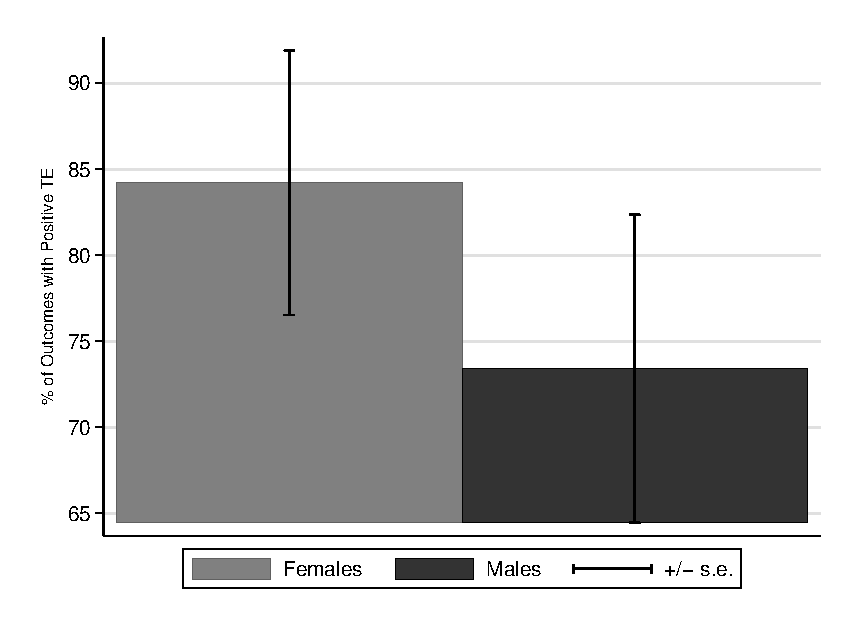
\includegraphics[width=20em]{output/itt_noctrl_all.eps}
\end{figure}
$\rightarrow$ Strengthen when accounting for substitution bias
\end{frame}

%% ---------------------------------------------------------------------------

\begin{frame}
\frametitle{Preview of Results: Cost-benefit Analysis}
	\begin{itemize}
		\item Monetize multiple dimensions of life-cycle costs and benefits \\
			$\rightarrow$ Costs: program, alternative preschool, education \\ 
			$\rightarrow$ Benefits: reduced special education; parental income; labor income; judicial, incarceration, and victimization costs; health expenditures; quality-adjusted life years 
	\end{itemize}
	\begin{center}
	\scalebox{.75}{\begin{tabular}{l c c c c c c }
\toprule
	&	\mc{2}{c}{Females}					&	\mc{2}{c}{Males}					&	\mc{2}{c}{Pooled}					\\
		\cmidrule(lr){2-3}						\cmidrule(lr){4-5}						\cmidrule(lr){6-7}					
Estimate 	&	IRR	&	B/C	&	IRR	&	B/C	&	IRR	&	B/C	\\
\midrule

% INSERT summary_tex.xls FILE BELOW
% INSERT summary_tex.xls FILE BELOW
% INSERT summary_tex.xls FILE BELOW

Baseline	&	0.10 	&	2.30	&	0.15 &	7.88 	&	\textbf{0.13}	&	\textbf{4.35}	\\
	&	(0.12)	&	(1.56)	&	(0.13)	&	(8.06)	&	(0.11)	&	(2.57)	\\
Relative to Staying at Home	&	-0.14	&	\textbf{4.97}	&	0.02	&	0.55	&	\textbf{0.09} &	3.78	\\
	&	(0.13)	&	(2.02)	&	(0.13)	&	(3.00)	&	(0.05)	&	(2.15)	\\
Relative to Alternative Preschools	&	0.08		&	1.58	&	\textbf{0.20}	&	\textbf{12.24}	&	\textbf{0.12}	&	4.34	\\
	&	(0.14)	&	(1.20)	&	(0.14)	&	(5.39)	&	(0.09)	&	(2.67)	\\

% INSERT summary_tex.xls FILE ABOVE
% INSERT summary_tex.xls FILE ABOVE
% INSERT summary_tex.xls FILE ABOVE

\bottomrule
\end{tabular}}
	\end{center}	
\end{frame}

%% ---------------------------------------------------------------------------

\begin{frame}
\frametitle{Preview of Results: Importance of Accounting for Long-term Effects}
\begin{figure}
\caption{Benefit-cost Ratio When Accounting for Benefits at Different Ages}
	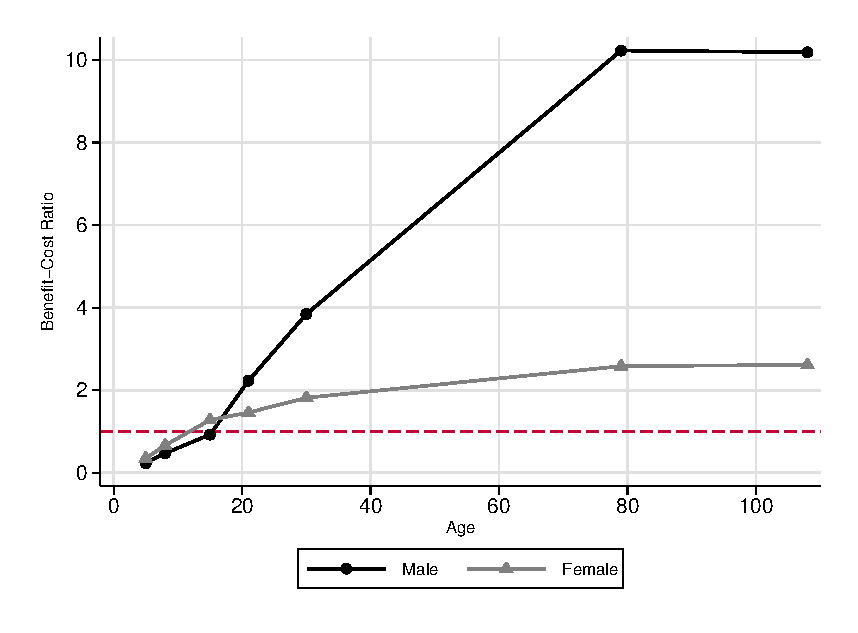
\includegraphics[width=16em]{AppOutput/Sensitivity/bcr_age.eps}
\end{figure}
\begin{itemize}
	\item The pooled benefit-cost ratio is 0.59 at age 5, 2.69 at age 30, and 4.3 at age 79
\end{itemize}
\end{frame}

\section{Data}

\begin{frame}[noframenumbering]

\begin{block}{}
\begin{center}
\textbf{Data}
\end{center}
\end{block}

\end{frame}

%% ---------------------------------------------------------------------------

\begin{frame}
\frametitle{Experimental Data}
\begin{table}
\footnotesize\caption{Data Availability for ABC and CARE (Part I)} \label{tab:datasumm_1}
\centering
\tiny
\begin{tabular*}{\textwidth}{L{4.8cm} C{2cm} C{2cm} C{2cm}} \toprule
Category & Age 0-5 & Age 5-15 & Adult  \\
\midrule
\textbf{Physical Health} \\
\quad Growth data & \CheckmarkBold & - & - \\
\quad Health issues & - & \CheckmarkBold  & \CheckmarkBold \\
\quad Full medical sweep & - & -  & \CheckmarkBold \\
 \midrule
\textbf{Family Environment} \\
\quad Family Members & \CheckmarkBold & \CheckmarkBold & \CheckmarkBold \\
\quad Economic Environment & \CheckmarkBold & \CheckmarkBold & \CheckmarkBold \\
\quad Family Social Status & \CheckmarkBold & \CheckmarkBold & - \\
\quad Family Physical Health & \CheckmarkBold & \CheckmarkBold & - \\
\quad Marital Status/Number of Children & - & - & \CheckmarkBold \\
 \midrule
\textbf{Childcare} \\
\quad Daycare/Parental Care Info & \CheckmarkBold & - & - \\
 \midrule
\textbf{Cognitive Assessments} \\
\quad Intelligence Levels & \CheckmarkBold & \CheckmarkBold & Only ABC \\
\quad Language Ability & \CheckmarkBold & \CheckmarkBold & - \\
\quad Motor Development & \CheckmarkBold & \CheckmarkBold & - \\
\quad Critical Thinking & Only ABC & \CheckmarkBold & - \\
 \bottomrule
\end{tabular*}
\end{table}
\end{frame}

%% ---------------------------------------------------------------------------

\begin{frame}
\frametitle{Experimental Data}
\begin{table}
\caption{Data Availability for ABC and CARE (Part II)} \label{tab:datasumm_2}
\centering
\tiny
\begin{tabular*}{\textwidth}{L{4.5cm} C{2cm} C{2cm} C{2cm}} \toprule
Category & Age 0-5 & Age 5-15  & Adult \\
\midrule
\textbf{Non-Cognitive Assessments} \\
\quad Social Skills & \CheckmarkBold & \CheckmarkBold & \CheckmarkBold \\
\quad Self Control & \CheckmarkBold & \CheckmarkBold & Only ABC \\
\quad Self-Consciousness & Only ABC & \CheckmarkBold & - \\
\quad Work Ethic & - & \CheckmarkBold & - \\
\quad Social Activities & - & \CheckmarkBold & \CheckmarkBold \\
 \midrule
\textbf{Academic Achievements} \\
\quad Standardized Tests & - & \CheckmarkBold & - \\
\quad Performance in School & - & \CheckmarkBold & - \\
\quad Education Level & - & - & \CheckmarkBold \\
 \midrule
\textbf{Economic Status} \\
\quad Living Circumstances & - & - & \CheckmarkBold \\
\quad Income/Working Condition & - & - & \CheckmarkBold \\
 \midrule
\textbf{Social Conduct} \\
\quad Administrative Criminal Records & - & - & \CheckmarkBold \\
\quad Law Breaking & - & \CheckmarkBold & \CheckmarkBold \\
\quad Smoking, Drinking, and Drugs & - & - & \CheckmarkBold \\
\bottomrule
\end{tabular*}
\end{table}
\end{frame}

%% ---------------------------------------------------------------------------

\begin{frame}
\frametitle{ABC First-phase Randomization Compromises and Attrition}

\begin{itemize}
\item Treatment group (59); Control group (57)
	\item Data on non-compliers available up to age 8: analyses accounting for these indicate insensitivity
	\item Account for attrition using inverse probability weighting \\
	$\rightarrow$ Based on conditional independence \citep{Horvitz_Thompson_1952_JASA}
\end{itemize}
\end{frame}

%% ---------------------------------------------------------------------------

\begin{frame}[noframenumbering]
\frametitle{ABC First-phase Randomization Compromises and Attrition}
\begin{center}
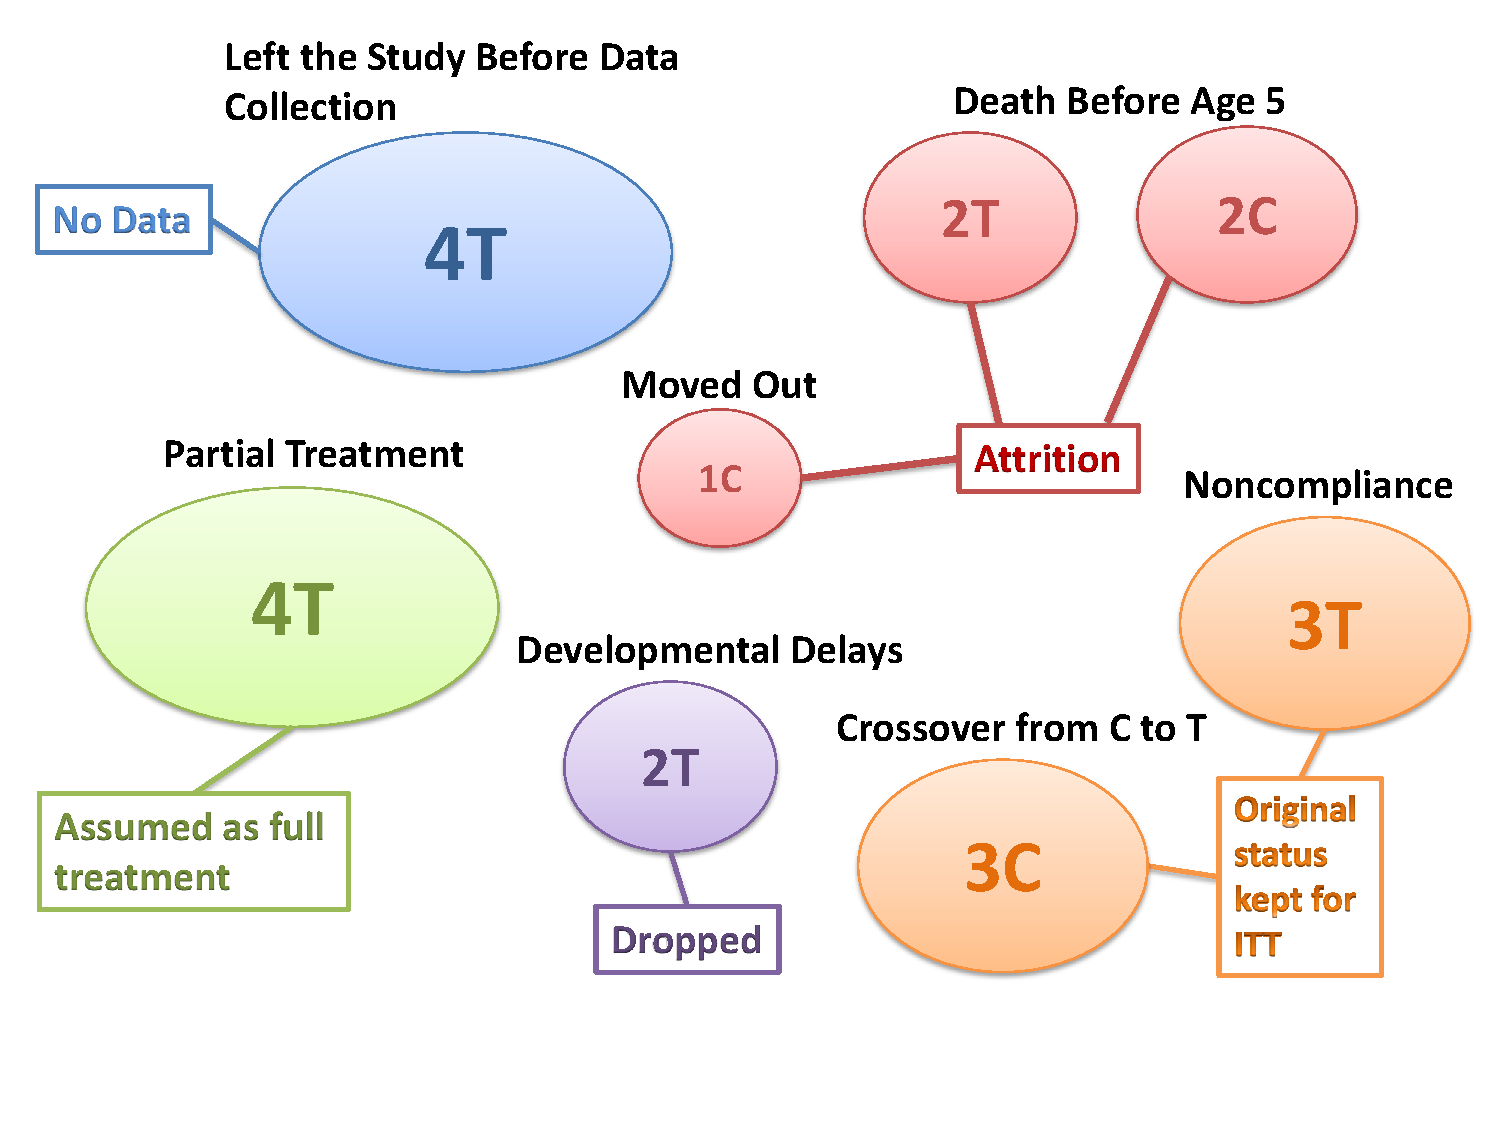
\includegraphics[scale=0.35]{images/abc_p1_randomization.pdf}
\end{center}
\end{frame}

%% ---------------------------------------------------------------------------

\begin{frame}
\frametitle{Auxiliary Data Sources}
\mode<presentation>{\begin{footnotesize}}
\begin{itemize}
	\item Auxiliary data used to construct life-cycle profiles:
	\begin{enumerate}\mode<presentation>{\begin{footnotesize}}
		\item Spans the life cycle
		\item Years of birth of the auxiliary sample match those of ABC
		\item Common support in predictors of outcome \mode<presentation>{\end{footnotesize}}
	\end{enumerate}
\end{itemize}
\begin{center}
	Auxiliary Sources for Interpolation and Extrapolation
	%\input{../../AuxilliaryFiles/Preamble}
%\newgeometry{margin=.1in}

%\newcolumntype{L}[1]{>{\raggedright\let\newline\\\arraybackslash\hspace{0pt}}m{#1}}
%\newcolumntype{C}[1]{>{\centering\let\newline\\\arraybackslash\hspace{0pt}}m{#1}}
%\newcolumntype{R}[1]{>{\raggedleft\let\newline\\\arraybackslash\hspace{0pt}}m{#1}}

\begin{tabular}{L{3cm} C{1cm} C{1cm} C{1cm} C{1cm} C{1cm} C{2cm}} \toprule
 & \multicolumn{6}{c}{Subject's Age} \\
\textbf{Component}  & 16--21 & 21--30 & 31--34 & 34--50 & 61--67 & 68--Death \\ \midrule
\textbf{Transfer Income} & & \multicolumn{1}{c}{\cellcolor[gray]{.8} cNLSY} & \multicolumn{3}{c}{\cellcolor[gray]{.7} NLSY79; PSID}  &  \\ \midrule
\textbf{Subject Income} & &  \multicolumn{1}{c}{\cellcolor[gray]{.8} cNLSY} & \multicolumn{3}{c}{\cellcolor[gray]{.7} NLSY79; PSID} & \\ \midrule
\textbf{Health}  & \multicolumn{6}{c}{\cellcolor[gray]{.8} PSID; MEPS; MCBS; HRS}     \\ \midrule
\textbf{Crime} & \multicolumn{4}{c}{\cellcolor[gray]{.8} NCDPS; NJRP; NVS; UCRS} \\ \bottomrule
\end{tabular}
%\end{document}
\end{center}
\mode<presentation>{\end{footnotesize}}
\end{frame}

%% ---------------------------------------------------------------------------

\section{Methodology}

\begin{frame}[noframenumbering]

\begin{block}{}
\begin{center}
\textbf{Methodology}
\end{center}
\end{block}

\end{frame}

%% ---------------------------------------------------------------------------

\begin{frame}
\frametitle{Evaluation Framework}
\begin{itemize}
	\item Let $\Omega$ be a set with $\sigma$-algebra $\sigma(\Omega)$; $\omega \in \Omega$ \\
	\begin{scriptsize}
		$\rightarrow$ $Y^1 \left( \omega \right)     $: treatment outcome  \\ 
		$\rightarrow$ $Y_H^0 \left(\omega \right)  $: control outcome staying at home \\
		$\rightarrow$ $Y_C^0 \left( \omega \right) $: control outcome in an alternative preschool
	\end{scriptsize}
	    \item $D=1$ indicates desire to participate of the program
	    \item  $R | D =1 $ random variable; randomization in or out treatment
	    \item Assume discrete temporal dimension; $T$ periods
		\item $V$: proportion of months in alternative preschool \\
		$\rightarrow$ Crude summary of likely more complex dynamics
\end{itemize}
\begin{equation}
	V(\omega)  : = \frac{\# \{ t : Y_H^0 \left( t, \omega \right) - Y_C^0 \left( t, \omega \right)  \leq 0 \}}{T}
\end{equation}

\begin{itemize}
	\item Counterfactual outcomes: \\
	$\rightarrow$ Assume $Y_H^0 \left( t,\omega \right) = Y_H^0 \left( \omega \right); Y_C^0\left(t,\omega\right)=Y_C^0\left(\omega\right)$ 
\end{itemize}

\begin{equation}
Y^0 \left( \omega \right) := \left[ 1 - V\left( \omega \right) \right] Y_H^0 \left( \omega \right)  +  V\left( \omega \right) Y_C^0 \left( \omega \right)   
\end{equation}
\end{frame}

%% ---------------------------------------------------------------------------

\begin{frame}
\frametitle{Control-group Substitution, ABC}\label{t_abc_substitution}
\begin{figure}
\caption{Months in Alternative Preschools, ABC Control Group}
	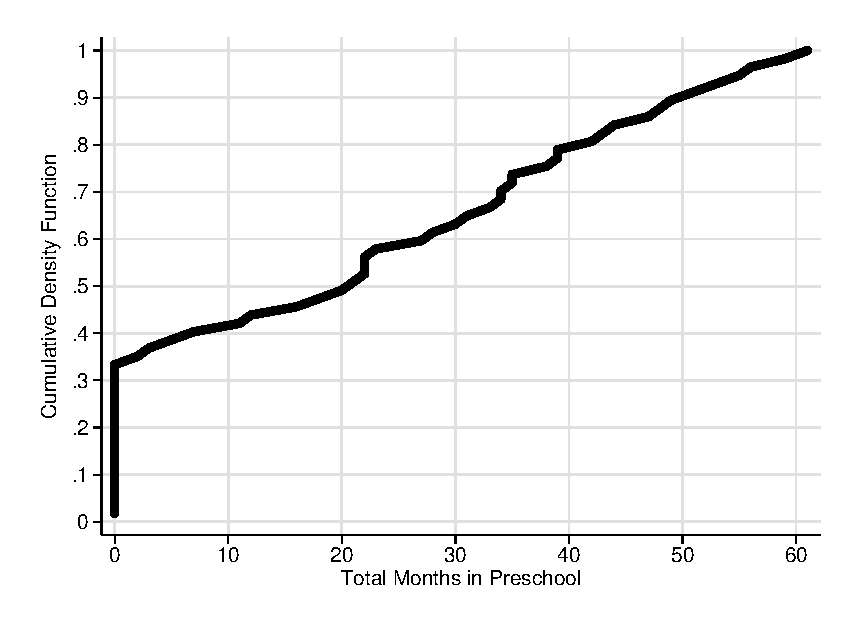
\includegraphics[width=20em]{output/abc_controlcontamination_months.eps}
\end{figure}
\hyperlink{abc_subsidized}{\beamergotobutton{Proportion Subsidized}}
\end{frame}

%% ---------------------------------------------------------------------------

\begin{frame}
\frametitle{Control-group Substitution, CARE}\label{t_care_substitution}
\begin{figure}
\caption{Months in Alternative Preschools, CARE}
	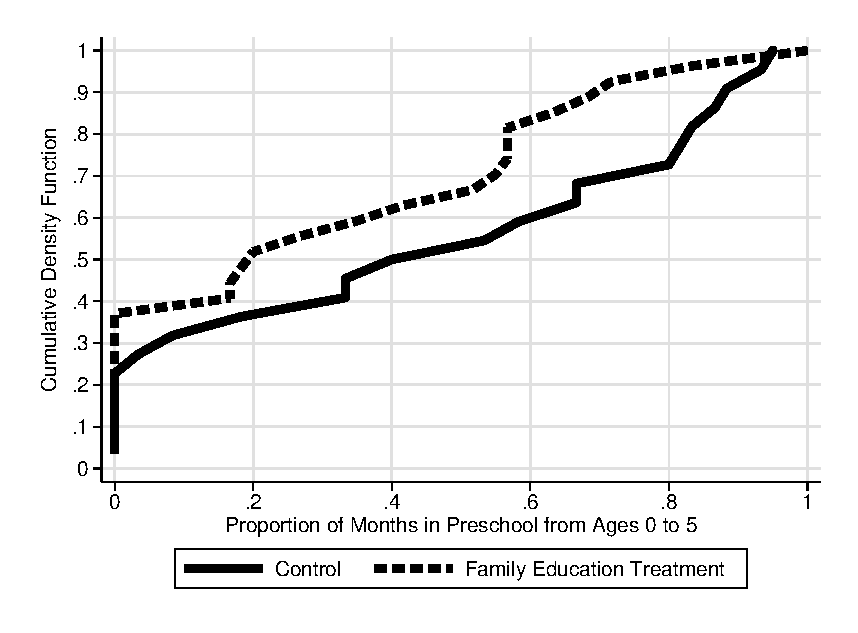
\includegraphics[width=20em]{output/care_controlcontamination_months.eps}
\end{figure}
\hyperlink{care_subsidized}{\beamergotobutton{Proportion Subsidized}}
\end{frame}

%% ---------------------------------------------------------------------------

\begin{frame}
\frametitle{Evaluation Framework}
\begin{itemize}
	\item Two possible approaches: \\
		$\rightarrow$ Multiple values for $V$ (possibly continuous in the limit) \\
		$\rightarrow$ Or restrict to binary values of $V$:  ($V=0$, $V>0$)
	\item Consider a Roy-type setting
	\item In our samples, treatment is preferred to either non-treatment outcomes: 
\end{itemize}

	\begin{equation}
		\Pr \left( Y^1 (\omega)  \geq \max \left( Y_H^0  (\omega) , Y_C^0  (\omega)\right)  | D = 1 \right) = 1
	\end{equation}
$\rightarrow$ Could instead use utilities over outcomes--e.g. $U \left( Y^1(\omega) \right)$
\begin{itemize}
	\item Various methods to identify and estimate the marginal distributions of $Y_H^0, Y_C^0$ \\
	$\rightarrow$ Problematic to utilize in a small sample setting 
	\item Ideally, construct counterfactual $Y_C^0 \left( v, \omega \right)$ for $v \in [0,1]$ \\
	$\rightarrow$ Difficult in small samples
\end{itemize}
\end{frame}

\begin{frame}
\frametitle{Counterfactual Comparisons}
\begin{itemize}
	\item Alternative evaluation counterfactuals  \\
\end{itemize}
		$\rightarrow$ Standard version: 

\begin{equation}
\Delta : = \mathbb{E}_{\Omega} \left[ Y^1 - max \left( Y_{H}^0, Y_C^0 \right)  | D = 1\right] 
\end{equation}

\begin{itemize}
	\item Evaluate relative to no control-group alternatives take-up
\end{itemize}

\begin{equation}
\Delta \left( v = 0 \right) := \mathbb{E}_{\Omega} \left[ Y^1\left( v \right) - Y^0\left( v \right) | V = 0, D = 1 \right]
\end{equation}

$\rightarrow$ Estimator:

\begin{eqnarray}
\widehat{\Delta} \left( v = 0 \right) &:=& \widehat{\mathbf{E}} \left[ Y | D = 1, R = 1, V \in [0,  \eta] \right] \nonumber \\ 
&-& \widehat{\mathbf{E}} \left[ Y | D = 1, R = 0,  V \in [0, \eta] \right]
\end{eqnarray}

with $\eta \rightarrow 0$

\begin{itemize}
\item $\Delta \left( v > 0 \right)$ analogously defined and estimated for $V > 0$
\end{itemize}
\end{frame}

\begin{frame}
\frametitle{Multiple Hypothesis Testing}
\begin{itemize}
\item Many outcomes \\
	$\rightarrow$ One possible procedure: step-down; blocks often arbitrary \\
    $\rightarrow$ Another possible procedure: combine all the treatment effects in a single statistic

\begin{itemize}	
	\item $\mathcal{G}$: index set for groups of outcomes
	\item $\mathcal{O}_g$: group of outcomes; $g \in \mathcal{G}$; cardinality $\#\mathcal{O}_g$
	\item $F_{j,g}^r \left( y_g^r \right)$ marginal distribution of outcome $j$ in $\mathcal{O}_g$; treatment group $r \in \{0, 1\}$
	\item $\Delta_{j,g}$: treatment effect associated with outcome $j$ in $\mathcal{O}_g$ 
\end{itemize}	
\end{itemize}
$\rightarrow$ Recall:
\begin{equation}
\Delta_{j,g} : = \mathbb{E}_{\Omega} \left[ Y^1_{j,g} - max \left( Y_{j,g,H}^0, Y_{j,g,C}^0 \right)  | D = 1\right] 
\end{equation}
\end{frame}
%% ---------------------------------------------------------------------------

\begin{frame}
\frametitle{Counting Socially Positive Treatment Effects}

\begin{itemize}
	\item Null hypotheses of interest: 
\end{itemize}
		\begin{equation}
			H_{0}: F_{j,g}^0 = F_{j,g}^1, \ \ \forall \ j \in \mathcal{O}^g 
		\end{equation}

\begin{itemize}
	\item In practice, we test: 
\end{itemize}
		\begin{eqnarray}
		H_{0} &:&  \Delta_{j,g} = 0, \ \ \forall \ j \in \mathcal{O}^g  \nonumber \\
		\end{eqnarray}

\begin{itemize}	
		\item Statistic:
\end{itemize}
	\begin{equation}
		T_g = \sum _{j=1}^{\# \mathcal{O}_g} \mathbf{1} \left[ \widehat{\Delta}_{j,g} > 0\right] \label{eq:count1}
	\end{equation}

\begin{itemize}	
		\item Test analogous hypotheses and define analogous statistic for positive and significant treatment effects
\end{itemize}
	
\end{frame}

%% ---------------------------------------------------------------------------

\begin{frame}
\frametitle{Cost-benefit Methodology}
\begin{itemize}
	\item Monetize lifetime social costs and benefits generated by the programs: income, health, education, and crime
	\item Multiple challenges
		\begin{enumerate}
			\item Intermittent data collection 
			\item Collection only up to age 34
			\item Attrition in later follow-ups
		\end{enumerate}
	\item Interpolation and extrapolation using multiple sources of auxiliary data
	\item Two statistics of interest: \textbf{internal rate of return} and \textbf{benefit-cost ratio}
	\item Provide standard errors and sensitivity analysis to choices of parameters
\end{itemize}
\end{frame}

%% ---------------------------------------------------------------------------

\begin{frame}
\frametitle{Earnings Projections}

$\rightarrow$ Key component of cost-benefit analysis \\
$\rightarrow$ Simplify notation: suppress $D =1$ henceforth 

\begin{align}
	\mathbb{E}  \left[ Y | R = r, X = x, W = w, S = s\right]= \phi \left(r, x, w, s \right)
\end{align}
\begin{itemize}
	\item $Y$: an outcome of interest---we suppress subscript $t$ for time period
	\item $R$: an indicator for participation in treatment (given $D=1$)
	\item $X$: observed set of variables, possibly affected by treatment
	\item $W$: pre-program variables
	\item $S$: an indicator equal to 1 if data is ABC, 0 if auxiliary
\end{itemize}
\end{frame}

%% ---------------------------------------------------------------------------
\begin{frame}
\frametitle{Earnings Projections}
\begin{description}
	\item [\textbf{Assumption 1:}] Common support between auxiliary datasets and the analysis sample
\end{description}
\begin{align*}
	\sup \left( X | S = 1 \right) \subseteq \sup \left( X | S = 0 \right)
\end{align*}
\begin{description}
	\item [\textbf{Assumption 2:}] Effect of treatment is captured by $X$; $Y$ is (mean) independent of $R$ conditional on $S, X, W$
\end{description}
\begin{align*}
	& \mathbb{E} \left[ Y | R = r, X = x, W = w, S = s \right] \\ %= \phi \left( x_{r}, w \right)
	&= \mathbb{E} \left[ Y | X = x^{r}, W = w, S = s \right]
\end{align*}

\begin{itemize}
	\item $Y : = \left( R\right)  Y^1 + (1 - R)Y^0$; $Y^r:= Y| R = r$
	\item $x^r$: vector drawn from the distribution $X \mid R=r$
	\item $X$: can include proxies; factors for latent skills; lagged values of $Y$ 
\end{itemize}
\end{frame}

%% ---------------------------------------------------------------------------
\begin{frame}
\frametitle{Earnings Projections}
Let $*$ indicate that a random variable is unobserved
\begin{itemize}
	\item Auxiliary Dataset, $S = 0$:  $\left( Y, X, W, R^{*} \right)$
	\item Analysis Sample, $S = 1$:   $\left( Y^{*}, X, W, R \right)$
\end{itemize}
\begin{description}
	\item [\textbf{Assumption 3:}] $Y$ is independent of $S$ conditional on $X, W, R$
\end{description}
\begin{align*}
	&\mathbb{E} \left[ Y^{*} | R = r, X = x, W = w, S = 1 \right] \\
	&= \mathbb{E} \left[ Y | R^{*} = r, X = x, W = w, S = 0 \right] \text{ for } r = 0,1
\end{align*}
\end{frame}

%% ---------------------------------------------------------------------------

\begin{frame}
\frametitle{Earnings Projections}
\begin{description}
	\item [\textbf{Assumption 4:}] Errors, $\varepsilon$, are additively separable
\end{description}

\begin{equation}
	Y = \phi \left( R, X, W, S \right) + \varepsilon
\end{equation}

Account for forecasting errors
\begin{itemize}
	\item $\widehat{\varepsilon}$: forecasting error  
	\item How? Add back to projections residuals drawn with replacement within bootstraps
\end{itemize}
\end{frame}

%% ---------------------------------------------------------------------------

\begin{frame}
\frametitle{Earnings Projections}
We identify $\phi\left(R, X, W, S = 1\right)$ as follows:
\begin{align*}
	& \phi\left(R, X, W, S = 1\right) \\
	&= \mathbb{E} \left[ Y^{*} | R = r, X = x, W = w, S = 1 \right] \\
	&= \mathbb{E} \left[ Y | R^{*} = r, X = x, W = w, S = 0 \right]\\
	&= \mathbb{E} \left[ Y | X = x^{r}, W = w, S = 0 \right]\\
\end{align*}
We estimate the treatment effects on $\hat{Y}$
\begin{equation}
	\hat{Y} = \phi \left( R, X, W, S=1 \right) + \hat{\varepsilon}
\end{equation}

\end{frame}

%% ---------------------------------------------------------------------------

\begin{frame}
\frametitle{Monetizing Crime Outcomes}
\begin{itemize}
\item Two elements \\
	$\rightarrow$ Account for costs and benefits  up to age 35 \\
	$\rightarrow$ Extrapolate thereafter: similar methodology as used for income
\item Data on arrests \\
	$\rightarrow$ Administrative data up to age 35 \\
	$\rightarrow$ Self-reported up to age 30
\item Auxiliary datasets:
	\begin{itemize}
	\item National Victimization Survey (NVS)
	\item Uniform Crime Reports (UCR)
	\item North Carolina Department of Public Safety (NCDPS)
	\end{itemize}
\item Account for victimization inflation \\ 
	$\rightarrow$ Use NVS and the UCR to create a ratio of victims to arrests
\end{itemize}
\end{frame}

%% ---------------------------------------------------------------------------

\begin{frame}
\frametitle{Extrapolation of Health Outcomes}
\begin{itemize}
	\item Future America Model (FAM) \\
		$\rightarrow$ Non-experimental data to provide estimates of medical expenditure and QALYs \citep{Goldman_etal_2015_Future-America-Model}
	\item First-order Markov process \\
	$\rightarrow$ Estimate probability of an individual transitioning into a health state \\
	$\rightarrow$ Monetize each health state based on SES characteristics
	\item Feed income projections and simulate the estimated outcomes using Monte-Carlo simulations \\
	 $\rightarrow$ Model incorporates subjects' data on heart disease, cancer, hypertension, smoking, marriage, divorce, insurance type
	 \item We estimate medical expenditure for ages 16 to 79 and account for the improvement to quality-of-life (QALY)
\end{itemize}
\end{frame}

%% ---------------------------------------------------------------------------

\begin{frame} \label{costs}
\begin{table}
\begin{center}
\caption{Costs and Benefits Across the Life Cycle} 
\scalebox{0.48}{\begin{tabular}{L{4cm} C{3cm} C{3cm} C{3cm} C{3cm} C{3cm} C{1.5cm}}
\toprule
& \textbf{Preschool} & \textbf{School Age} & \textbf{Young Adult} & \textbf{Mid-30s} & \textbf{Midlife} & \textbf{Post-Retirement} \\
\midrule
\textbf{Program Costs} &  \cellcolor[gray]{.8}  Nutrition; medical costs; education & & & & & \\
\midrule
\textbf{Other Center-Based Education} & \cellcolor[gray]{.8}  Education; subsidies	& & & & & \\
\midrule
\textbf{Education} &	& \multicolumn{1}{C{3cm}|}{\cellcolor[gray]{.8}  Elementary to high school; grade retention; special education} 	&  \multicolumn{1}{C{3cm}|}{\cellcolor[gray]{.8} High school; GED; vocational; college} & \multicolumn{1}{C{3cm}}{\cellcolor[gray]{.8} Rest of education history} & & \\
\midrule
\textbf{Parental Income}	& \multicolumn{2}{c}{\cellcolor[gray]{.8} Total labor income} &  & & & \\
\midrule
\textbf{Welfare Income} &	& & \multicolumn{3}{c}{\cellcolor[gray]{.8}Total transfers received from government}	& \\
\midrule
\textbf{Subject Income} & & & \multicolumn{3}{c}{\cellcolor[gray]{.8}Total labor income} & \\
\midrule
\textbf{Health} & & & \multicolumn{4}{c}{\cellcolor[gray]{.8} Medical expenditures; quality-adjusted life years} \\
\midrule
\textbf{Crime} &	 & & \multicolumn{2}{c}{\cellcolor[gray]{.8} Prison; justice system; victimization costs} & \multicolumn{1}{|C{3cm}}{\cellcolor[gray]{.8} Prediction and imputation of crime sentence and justice system costs} & \\
\bottomrule
\end{tabular}}
\end{center}
\end{table}
\hyperlink{components}{\beamergotobutton{Detailed Components}}
\end{frame}

%% ---------------------------------------------------------------------------

\section{Empirical Estimates}

\begin{frame}[noframenumbering]

\begin{block}{}
\begin{center}
\textbf{Empirical Estimates}
\end{center}
\end{block}

\end{frame}

%% ---------------------------------------------------------------------------

\begin{frame}
\frametitle{Summary of Treatment Effects}
\begin{itemize}
	\item Males and Females: majority of outcomes display positive treatment effect 
	$\rightarrow$ More than 30\% are individually statistically significant at 10\% level
	\item Females: 
		\begin{itemize}
			\item Positive effects on outcomes related to cognitive skills and education
			\item Once control-group substitution is accounted for, results strengthen
		\end{itemize}
	\item Males:
		\begin{itemize}
			\item Positive effects on outcomes related to labor market performance and health
			\item Results are weaker with respect to step-down correction
		\end{itemize}
	\item Gender difference in impacted outcomes generates difference in benefit-cost calculation \\
		$\rightarrow$ Outcomes impacted for males have higher monetary value
	\end{itemize}
\end{frame}	

%% ---------------------------------------------------------------------------

\begin{frame} \label{resultsfemales}
\begin{table}
	\caption{ABC and CARE Females, Selected Outcomes}
	\scalebox{0.7}{  \begin{tabular}{cccccccc}
  \toprule

    \scriptsize{Variable} & \scriptsize{Age} & \scriptsize{(1)} & \scriptsize{(2)} & \scriptsize{(3)} & \scriptsize{(4)} & \scriptsize{(5)} & \scriptsize{(6)} \\ 
    \midrule  

    \mc{1}{l}{\scriptsize{Std. IQ Test}} & \mc{1}{c}{\scriptsize{12}} & \mc{1}{c}{\scriptsize{8.688}} & \mc{1}{c}{\scriptsize{7.857}} & \mc{1}{c}{\scriptsize{6.850}} & \mc{1}{c}{\scriptsize{6.441}} & \mc{1}{c}{\scriptsize{9.120}} & \mc{1}{c}{\scriptsize{8.429}} \\  

     &  & \mc{1}{c}{\scriptsize{\textbf{(0.000)}}} & \mc{1}{c}{\scriptsize{\textbf{(0.013)}}} & \mc{1}{c}{\scriptsize{\textbf{(0.026)}}} & \mc{1}{c}{\scriptsize{\textbf{(0.039)}}} & \mc{1}{c}{\scriptsize{\textbf{(0.000)}}} & \mc{1}{c}{\scriptsize{\textbf{(0.013)}}} \\  

    \mc{1}{l}{\scriptsize{Years of Edu.}} & \mc{1}{c}{\scriptsize{30}} & \mc{1}{c}{\scriptsize{2.143}} & \mc{1}{c}{\scriptsize{1.695}} & \mc{1}{c}{\scriptsize{4.025}} & \mc{1}{c}{\scriptsize{3.918}} & \mc{1}{c}{\scriptsize{1.567}} & \mc{1}{c}{\scriptsize{1.409}} \\  

     &  & \mc{1}{c}{\scriptsize{\textbf{(0.000)}}} & \mc{1}{c}{\scriptsize{\textbf{(0.000)}}} & \mc{1}{c}{\scriptsize{\textbf{(0.000)}}} & \mc{1}{c}{\scriptsize{\textbf{(0.000)}}} & \mc{1}{c}{\scriptsize{\textbf{(0.013)}}} & \mc{1}{c}{\scriptsize{\textbf{(0.026)}}} \\  

    \mc{1}{l}{\scriptsize{Public-Transfer Income}} & \mc{1}{c}{\scriptsize{30}} & \mc{1}{c}{\scriptsize{-2,672}} & \mc{1}{c}{\scriptsize{-1,560}} & \mc{1}{c}{\scriptsize{-3,053}} & \mc{1}{c}{\scriptsize{-3,213}} & \mc{1}{c}{\scriptsize{-2,269}} & \mc{1}{c}{\scriptsize{-2,620}} \\  

     &  & \mc{1}{c}{\scriptsize{\textbf{(0.026)}}} & \mc{1}{c}{\scriptsize{(0.118)}} & \mc{1}{c}{\scriptsize{\textbf{(0.013)}}} & \mc{1}{c}{\scriptsize{\textbf{(0.013)}}} & \mc{1}{c}{\scriptsize{(0.105)}} & \mc{1}{c}{\scriptsize{(0.132)}} \\  

    \mc{1}{l}{\scriptsize{Employed}} & \mc{1}{c}{\scriptsize{30}} & \mc{1}{c}{\scriptsize{0.131}} & \mc{1}{c}{\scriptsize{0.080}} & \mc{1}{c}{\scriptsize{0.333}} & \mc{1}{c}{\scriptsize{0.340}} & \mc{1}{c}{\scriptsize{0.056}} & \mc{1}{c}{\scriptsize{0.070}} \\  

     &  & \mc{1}{c}{\scriptsize{\textbf{(0.092)}}} & \mc{1}{c}{\scriptsize{(0.171)}} & \mc{1}{c}{\scriptsize{\textbf{(0.053)}}} & \mc{1}{c}{\scriptsize{\textbf{(0.053)}}} & \mc{1}{c}{\scriptsize{(0.276)}} & \mc{1}{c}{\scriptsize{(0.263)}} \\  

    \mc{1}{l}{\scriptsize{Total Years Incarcerated}} & \mc{1}{c}{\scriptsize{30}} & \mc{1}{c}{\scriptsize{-0.024}} & \mc{1}{c}{\scriptsize{-0.025}} &  &  & \mc{1}{c}{\scriptsize{-0.037}} & \mc{1}{c}{\scriptsize{-0.038}} \\  

     &  & \mc{1}{c}{\scriptsize{\textbf{(0.053)}}} & \mc{1}{c}{\scriptsize{\textbf{(0.066)}}} &  &  & \mc{1}{c}{\scriptsize{\textbf{(0.053)}}} & \mc{1}{c}{\scriptsize{\textbf{(0.066)}}} \\  

    \mc{1}{l}{\scriptsize{Diabetes}} & \mc{1}{c}{\scriptsize{Mid-30s}} & \mc{1}{c}{\scriptsize{-0.071}} & \mc{1}{c}{\scriptsize{-0.032}} &  &  & \mc{1}{c}{\scriptsize{-0.091}} & \mc{1}{c}{\scriptsize{-0.095}} \\  

     &  & \mc{1}{c}{\scriptsize{\textbf{(0.066)}}} & \mc{1}{c}{\scriptsize{(0.171)}} &  &  & \mc{1}{c}{\scriptsize{\textbf{(0.066)}}} & \mc{1}{c}{\scriptsize{\textbf{(0.039)}}} \\  

  \bottomrule
  \end{tabular}}
\end{table}
\begin{tiny}
\leftright{\textbf{(1)} $\mathbb{E}_\Omega \big[ Y^1(\omega) - Y^0(\omega) | D = 1\big]$}{\textbf{(4)} $\mathbb{E}_\Omega \big[ Y^1(v, \omega) - Y^0(v, \omega) | V=0, D = 1 \big] $} \par
\leftright{\textbf{(2)} $\mathbb{E}_\Omega \big[ Y^1(\omega) - Y^0(\omega) |  X, D = 1 \big]$}{\textbf{(5)} $\mathbb{E}_\Omega \big[ Y^1(\omega) \big] - \mathbb{E}_\Omega \big[ Y^0(v, \omega) | V > 0, D =1 \big]$} \par
\leftright{\textbf{(3)} $\mathbb{E}_\Omega \big[ Y^1(\omega) \big] - \mathbb{E}_\Omega \big[ Y^0(v, \omega) | V =0, D =1 \big]$}{\textbf{(6)} $\mathbb{E}_\Omega \big[ Y^1(v, \omega) - Y^0(v, \omega) | V > 0 , D = 1\big]$}

\end{tiny}
\hyperlink{stepdownfemales}{\beamergotobutton{Stepdown}}
\end{frame}

%% ---------------------------------------------------------------------------

\begin{frame} \label{resultsmales}
\begin{table}
	\caption{ABC and CARE Males, Selected Outcomes}
	\scalebox{0.7}{  \begin{tabular}{cccccccc}
  \toprule

    \scriptsize{Variable} & \scriptsize{Age} & \scriptsize{(1)} & \scriptsize{(2)} & \scriptsize{(3)} & \scriptsize{(4)} & \scriptsize{(5)} & \scriptsize{(6)} \\ 
    \midrule  

    \mc{1}{l}{\scriptsize{Years of Edu.}} & \mc{1}{c}{\scriptsize{30}} & \mc{1}{c}{\scriptsize{0.525}} & \mc{1}{c}{\scriptsize{0.708}} & \mc{1}{c}{\scriptsize{0.857}} & \mc{1}{c}{\scriptsize{0.791}} & \mc{1}{c}{\scriptsize{0.385}} & \mc{1}{c}{\scriptsize{0.347}} \\  

     &  & \mc{1}{c}{\scriptsize{\textbf{(0.079)}}} & \mc{1}{c}{\scriptsize{\textbf{(0.079)}}} & \mc{1}{c}{\scriptsize{(0.118)}} & \mc{1}{c}{\scriptsize{(0.171)}} & \mc{1}{c}{\scriptsize{(0.171)}} & \mc{1}{c}{\scriptsize{(0.276)}} \\  

    \mc{1}{l}{\scriptsize{Labor Income}} & \mc{1}{c}{\scriptsize{30}} & \mc{1}{c}{\scriptsize{19,810}} & \mc{1}{c}{\scriptsize{24,902}} & \mc{1}{c}{\scriptsize{17,909}} & \mc{1}{c}{\scriptsize{24,012}} & \mc{1}{c}{\scriptsize{20,065}} & \mc{1}{c}{\scriptsize{21,170}} \\  

     &  & \mc{1}{c}{\scriptsize{\textbf{(0.079)}}} & \mc{1}{c}{\scriptsize{(0.171)}} & \mc{1}{c}{\scriptsize{(0.132)}} & \mc{1}{c}{\scriptsize{(0.105)}} & \mc{1}{c}{\scriptsize{\textbf{(0.066)}}} & \mc{1}{c}{\scriptsize{(0.158)}} \\  

    \mc{1}{l}{\scriptsize{Employed}} & \mc{1}{c}{\scriptsize{30}} & \mc{1}{c}{\scriptsize{0.119}} & \mc{1}{c}{\scriptsize{0.179}} & \mc{1}{c}{\scriptsize{-0.029}} & \mc{1}{c}{\scriptsize{0.041}} & \mc{1}{c}{\scriptsize{0.176}} & \mc{1}{c}{\scriptsize{0.262}} \\  

     &  & \mc{1}{c}{\scriptsize{\textbf{(0.079)}}} & \mc{1}{c}{\scriptsize{\textbf{(0.039)}}} & \mc{1}{c}{\scriptsize{(0.487)}} & \mc{1}{c}{\scriptsize{(0.355)}} & \mc{1}{c}{\scriptsize{\textbf{(0.053)}}} & \mc{1}{c}{\scriptsize{\textbf{(0.000)}}} \\  

    \mc{1}{l}{\scriptsize{Total Misdemeanor Arrests}} & \mc{1}{c}{\scriptsize{Mid-30s}} & \mc{1}{c}{\scriptsize{-0.501}} & \mc{1}{c}{\scriptsize{-0.239}} & \mc{1}{c}{\scriptsize{-0.251}} & \mc{1}{c}{\scriptsize{-0.040}} & \mc{1}{c}{\scriptsize{-0.665}} & \mc{1}{c}{\scriptsize{-0.512}} \\  

     &  & \mc{1}{c}{\scriptsize{(0.132)}} & \mc{1}{c}{\scriptsize{(0.316)}} & \mc{1}{c}{\scriptsize{(0.408)}} & \mc{1}{c}{\scriptsize{(0.395)}} & \mc{1}{c}{\scriptsize{(0.105)}} & \mc{1}{c}{\scriptsize{(0.118)}} \\  

    \mc{1}{l}{\scriptsize{Diastolic Blood Pressure (mm Hg)}} & \mc{1}{c}{\scriptsize{Mid-30s}} & \mc{1}{c}{\scriptsize{-10.854}} & \mc{1}{c}{\scriptsize{-19.895}} & \mc{1}{c}{\scriptsize{-8.640}} & \mc{1}{c}{\scriptsize{-8.150}} & \mc{1}{c}{\scriptsize{-14.240}} & \mc{1}{c}{\scriptsize{-21.851}} \\  

     &  & \mc{1}{c}{\scriptsize{\textbf{(0.000)}}} & \mc{1}{c}{\scriptsize{\textbf{(0.000)}}} & \mc{1}{c}{\scriptsize{\textbf{(0.013)}}} & \mc{1}{c}{\scriptsize{\textbf{(0.026)}}} & \mc{1}{c}{\scriptsize{\textbf{(0.013)}}} & \mc{1}{c}{\scriptsize{\textbf{(0.000)}}} \\  

    \mc{1}{l}{\scriptsize{Vitamin D Deficiency}} & \mc{1}{c}{\scriptsize{Mid-30s}} & \mc{1}{c}{\scriptsize{-0.245}} & \mc{1}{c}{\scriptsize{-0.185}} & \mc{1}{c}{\scriptsize{-0.480}} & \mc{1}{c}{\scriptsize{-0.485}} & \mc{1}{c}{\scriptsize{-0.172}} & \mc{1}{c}{\scriptsize{-0.189}} \\  

     &  & \mc{1}{c}{\scriptsize{\textbf{(0.066)}}} & \mc{1}{c}{\scriptsize{(0.132)}} & \mc{1}{c}{\scriptsize{\textbf{(0.000)}}} & \mc{1}{c}{\scriptsize{\textbf{(0.000)}}} & \mc{1}{c}{\scriptsize{(0.158)}} & \mc{1}{c}{\scriptsize{(0.158)}} \\  

    \mc{1}{l}{\scriptsize{Self-reported drug user}} & \mc{1}{c}{\scriptsize{Mid-30s}} & \mc{1}{c}{\scriptsize{-0.333}} & \mc{1}{c}{\scriptsize{-0.432}} & \mc{1}{c}{\scriptsize{-0.500}} & \mc{1}{c}{\scriptsize{-0.555}} & \mc{1}{c}{\scriptsize{-0.233}} & \mc{1}{c}{\scriptsize{-0.330}} \\  

     &  & \mc{1}{c}{\scriptsize{\textbf{(0.026)}}} & \mc{1}{c}{\scriptsize{\textbf{(0.000)}}} & \mc{1}{c}{\scriptsize{\textbf{(0.000)}}} & \mc{1}{c}{\scriptsize{\textbf{(0.000)}}} & \mc{1}{c}{\scriptsize{(0.118)}} & \mc{1}{c}{\scriptsize{\textbf{(0.039)}}} \\  

  \bottomrule
  \end{tabular}}
\end{table}
\begin{tiny}
\leftright{\textbf{(1)} $\mathbb{E}_\Omega \big[ Y^1(\omega) - Y^0(\omega) | D = 1\big]$}{\textbf{(4)} $\mathbb{E}_\Omega \big[ Y^1(v, \omega) - Y^0(v, \omega) | V=0, D = 1 \big] $} \par
\leftright{\textbf{(2)} $\mathbb{E}_\Omega \big[ Y^1(\omega) - Y^0(\omega) |  X, D = 1 \big]$}{\textbf{(5)} $\mathbb{E}_\Omega \big[ Y^1(\omega) \big] - \mathbb{E}_\Omega \big[ Y^0(v, \omega) | V > 0, D =1 \big]$} \par
\leftright{\textbf{(3)} $\mathbb{E}_\Omega \big[ Y^1(\omega) \big] - \mathbb{E}_\Omega \big[ Y^0(v, \omega) | V =0, D =1 \big]$}{\textbf{(6)} $\mathbb{E}_\Omega \big[ Y^1(v, \omega) - Y^0(v, \omega) | V > 0 , D = 1\big]$}

\end{tiny}
\hyperlink{stepdownmales}{\beamergotobutton{Stepdown}}
\end{frame}

%% ---------------------------------------------------------------------------

\begin{frame}
\begin{figure}
\caption{Proportion of Outcomes with a Positive Treatment Effect}
	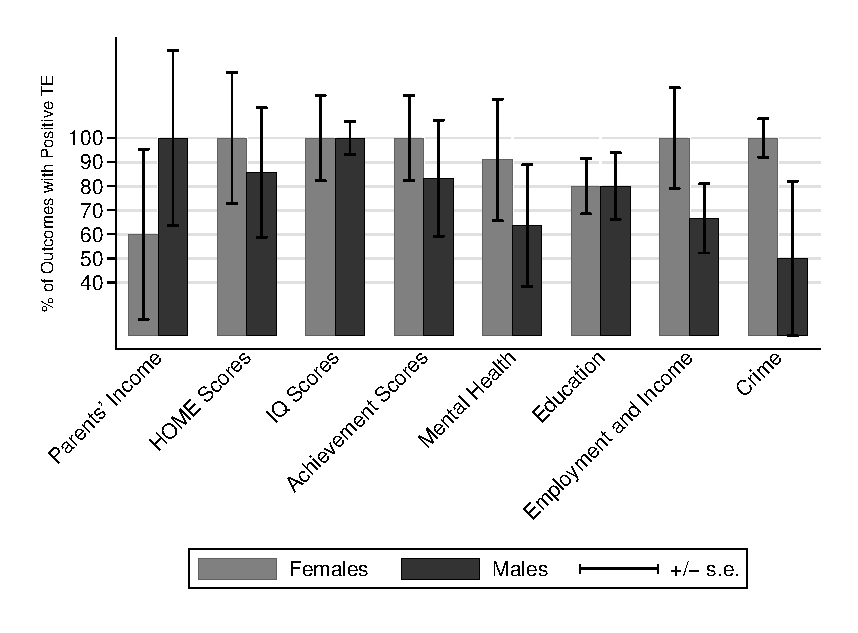
\includegraphics[width=20em]{output/itt_noctrl_cats1.eps}
\end{figure}
\end{frame}

%% ---------------------------------------------------------------------------

\begin{frame}
\begin{figure}
\caption{Proportion of Outcomes with a Positive Treatment Effect}
	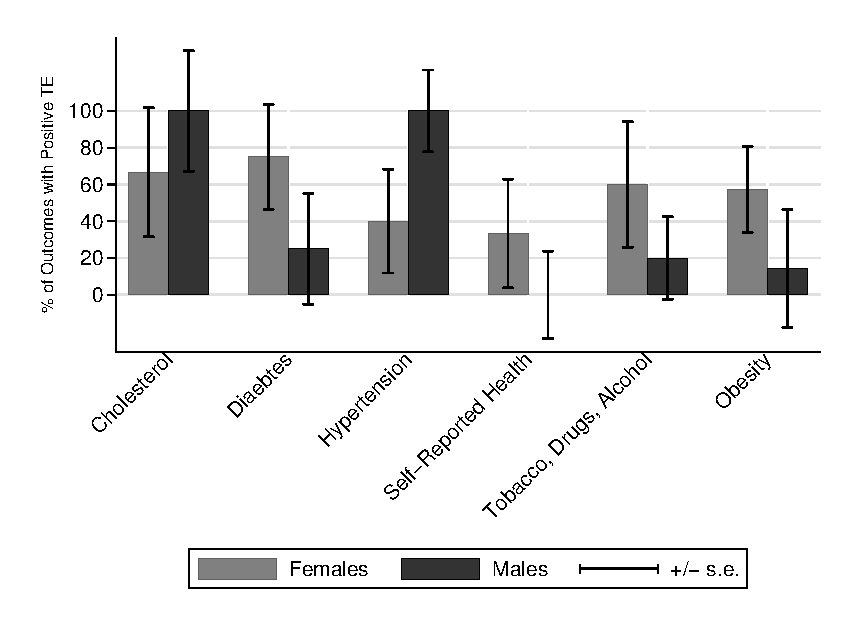
\includegraphics[width=20em]{output/itt_noctrl_cats2.eps}
\end{figure}
\end{frame}

%% ---------------------------------------------------------------------------

\begin{frame}
\begin{figure}
\caption{Proportion of Outcomes with a Positive and Significant Treatment Effect, at 10\% Level}
	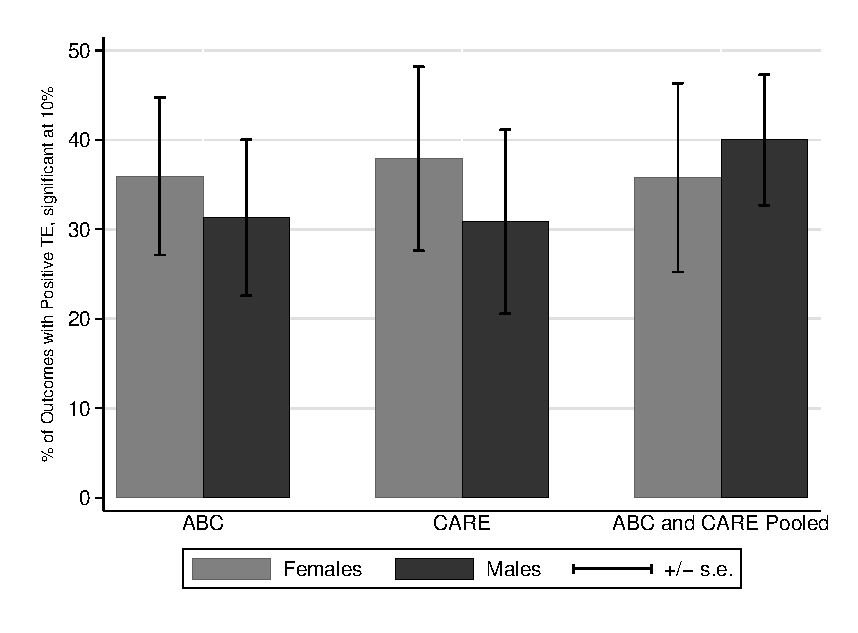
\includegraphics[width=20em]{output/itt_noctrl_all_sig10.eps}
\end{figure}
\end{frame}

%% ---------------------------------------------------------------------------

\begin{frame}\label{epan_ipw_p0_all}
\begin{figure}
\caption{Proportion of Outcomes with a Positive Treatment Effect Fixing Control Group to No Alternative Preschool}
	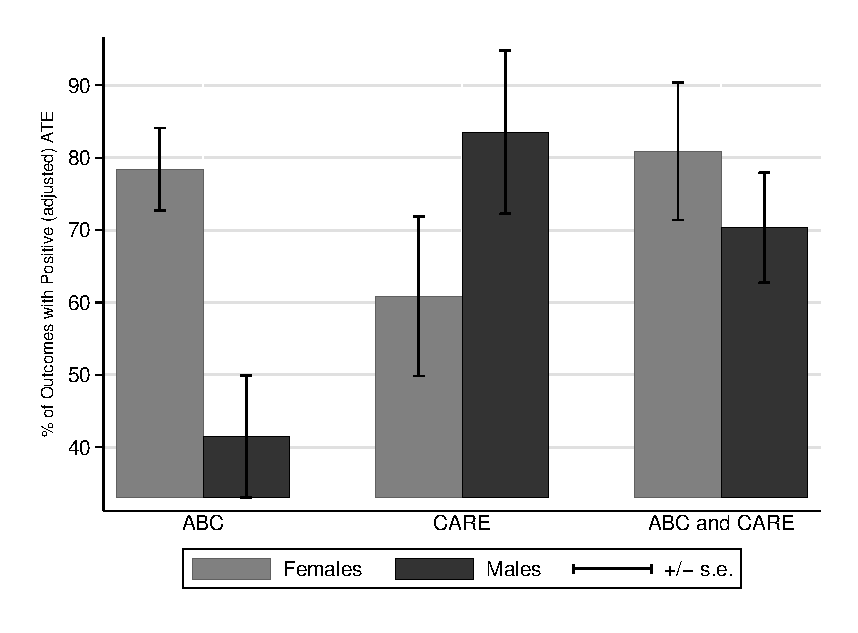
\includegraphics[width=20em]{output/epan_ipw_p0_all.eps}
\end{figure}
\end{frame}

%% ---------------------------------------------------------------------------

\begin{frame}
\frametitle{Monetizing the Costs and Benefits Treatment Effects}
\begin{itemize}
	\item We estimate the following:
	\begin{itemize} 
		\item Net Present Value (NPV) in 2014 USD, discounted at 3\% per year until birth
		\item Internal Rate of Return (IRR)
		\item Benefit-Cost Ratio (B/C) 
	\end{itemize}
	\item Standard errors are presented in parentheses and obtained using bootstrapping
	\begin{itemize}
		\item 200 resamples of ABC
		\item 200 resamples of auxiliary data
	\end{itemize}
	\item Point estimates in bold are significant at the 10\% level in a one-sided test 

\end{itemize}
\end{frame}

%% ---------------------------------------------------------------------------
\begin{frame}
\frametitle{Results and Sensitivity Analysis}
\begin{center}
\begin{table}
	\caption{Benefit-Cost Ratio and Rate of Return} \label{tab:bcr_irr1}
	\scalebox{.45}{\begin{tabular}{l r r r r r r r r r}																			
\toprule																			
&       \mc{3}{c}{Females}      &       \mc{3}{c}{Males}        &       \mc{3}{c}{Pooled}       \\																			
\cmidrule(lr){2-4}      \cmidrule(lr){5-7}      \cmidrule(lr){8-10}																			
Removed Component       &       NPV     &       IRR     &       B/C     &       NPV     &       IRR     &       B/C     &       NPV     &       IRR     &       B/C     \\																			
\midrule																			
None	&	161,759	&	\textbf{10.1\%}	&	\textbf{2.61}	&	919,049	&	\textbf{14.7\%}	&	\textbf{10.19}	&	636,674	&	\textbf{13.7\%}	&	\textbf{7.33}	\\
	&		&	(6\%)	&	(0.73)	&		&	(4\%)	&	(2.93)	&		&	(3\%)	&	(1.84)	\\ \\
Parental Income	&	148,854	&	4\%	&	1.12	&	107,907	&	\textbf{11\%}	&	\textbf{9.10}	&	116,953	&	\textbf{9\%}	&	\textbf{6.17}	\\
	&		&	(2\%)	&	(0.65)	&		&	(3\%)	&	(2.92)	&		&	(3\%)	&	(1.87)	\\
Subject Labor Income	&	41,908	&	9\%	&	\textbf{2.21}	&	238,105	&	\textbf{13\%}	&	\textbf{7.75}	&	133,032	&	\textbf{13\%}	&	\textbf{6.03}	\\
	&		&	(6\%)	&	(0.66)	&		&	(5\%)	&	(2.23)	&		&	(4\%)	&	(1.77)	\\
Subject Transfer Income	&	419	&	\textbf{10\%}	&	\textbf{2.61}	&	-7,265	&	\textbf{15\%}	&	\textbf{10.26}	&	-4,372	&	\textbf{14\%}	&	\textbf{7.38}	\\
	&		&	(6\%)	&	(0.73)	&		&	(4\%)	&	(2.93)	&		&	(3\%)	&	(1.84)	\\
Subject QALY	&	42,102	&	9\%	&	\textbf{2.20}	&	106,218	&	\textbf{14\%}	&	\textbf{9.14}	&	87,181	&	\textbf{13\%}	&	\textbf{6.48}	\\
	&		&	(6\%)	&	(0.69)	&		&	(6\%)	&	(2.73)	&		&	(5\%)	&	(1.79)	\\
Medical Expenditures	&	-16,037	&	9\%	&	\textbf{2.77}	&	-42,038	&	\textbf{15\%}	&	\textbf{10.61}	&	-31,221	&	\textbf{14\%}	&	\textbf{7.65}	\\
	&		&	(6\%)	&	(0.76)	&		&	(3\%)	&	(2.89)	&		&	(3\%)	&	(1.85)	\\
Alternative Preschools	&	16,691	&	8\%	&	\textbf{2.45}	&	13,434	&	\textbf{14\%}	&	\textbf{10.05}	&	14,659	&	\textbf{12\%}	&	\textbf{7.19}	\\
	&		&	(5\%)	&	(0.73)	&		&	(4\%)	&	(2.92)	&		&	(3\%)	&	(1.84)	\\
Education Costs	&	1,457	&	\textbf{10\%}	&	\textbf{2.59}	&	-7,852	&	\textbf{15\%}	&	\textbf{10.26}	&	-4,518	&	\textbf{14\%}	&	\textbf{7.37}	\\
	&		&	(6\%)	&	(0.72)	&		&	(4\%)	&	(2.93)	&		&	(3\%)	&	(1.86)	\\
Crime Costs	&	31,668	&	10\%	&	\textbf{2.34}	&	638,923	&	\textbf{9\%}	&	4.08	&	450,368	&	\textbf{8\%}	&	\textbf{3.06}	\\
	&		&	(6\%)	&	(0.62)	&		&	(5\%)	&	(2.18)	&	&	(4\%)	&	(1.01)	\\ \\
Deadweight Loss	&		&	\textbf{18\%}	&	\textbf{3.83}	&		&	\textbf{19\%}	&	\textbf{15.38}	&		&	\textbf{18\%}	&	\textbf{11.01}	\\
	&		&	(12\%)	&	(1.04)	&		&	(6\%)	&	(4.35)	&		&	(5\%)	&	(2.79)	\\
0\% Discount Rate	&		&		&	\textbf{5.06}	&		&		&	\textbf{25.45}	&		&		&	\textbf{17.40}	\\
	&		&		&	(2.82)	&		&		&	(10.42)	&		&		&	(5.90)	\\
7\% Discount Rate	&		&		&	\textbf{1.49}	&		&		&	\textbf{3.78}	&		&		&	\textbf{2.91}	\\
	&		&		&	(0.32)	&		&		&	(0.79)	&		&		&	(0.59)	\\
\bottomrule																			
\end{tabular}																			
}
\end{table}
\end{center}
\end{frame}
\clearpage



%% ----------------------------Appendix slides-----------------------------------------------

\appendix
\backupbegin
%\section*{Appendix}
\begin{frame}[noframenumbering]

\begin{block}{}
\begin{center}
\textbf{Appendix}
\end{center}
\end{block}

\end{frame}

%% ---------------------------------------------------------------------------

\begin{frame} \label{secondphase}
\frametitle{First-phase Treatment, ABC}
\begin{itemize}
	\item First-phase Treatment, ABC: one control group and one treatment group
		\begin{itemize}
			\item Control group (57 children):
				\begin{enumerate}								
				 \item Iron-fortified formula and monthly supply of diapers, first 15 months of life
				\end{enumerate} 
			\item Treatment group (59 children): 
				\begin{enumerate}
				\item Iron-fortified formula and monthly supply of diapers, first 15 months of life
				\item Breakfast, lunch, and afternoon snack
				\item Medical care from nurses, supervised by a doctor
				\item Center-based childcare
				\end{enumerate}
		\end{itemize}			
\end{itemize}
\hyperlink{programs}{\beamergotobutton{Back}}
\end{frame}

%% ---------------------------------------------------------------------------

\begin{frame}
\frametitle{First-phase Treatment, CARE}
\begin{itemize}
	\item First-phase Treatment, CARE: one control group and two treatment groups
		\begin{itemize}
			\item Control group (23 children):
				\begin{enumerate}								
				 \item Iron-fortified formula and monthly supply of diapers, first 15 months of life
				\end{enumerate} 
			\item Family education treatment group (27 children)
				\begin{enumerate}
				 \item Iron-fortified formula and monthly supply of diapers, first 15 months of life
				 \item Home visits that aimed to help parents solve common problems related to child rearing. 
				\end{enumerate}
			\item Center-based childcare and family education treatment group (16 children): 
				\begin{enumerate}
					\item Same as the family education treatment group
					\item Center-based childcare	
				\end{enumerate}							
		\end{itemize}
	\end{itemize}
\hyperlink{programs}{\beamergotobutton{Back}}
\end{frame}

%% ---------------------------------------------------------------------------


\begin{frame}

\frametitle{Second-phase Treatment, ABC and CARE}

\begin{itemize}

	\item For both programs: home visits from ages 5 to 8 \\

		$\rightarrow$ similar in objectives to first-phase home visits of CARE

	\item ABC: re-randomized at age 5 to either receive or not the home visits \\

	$\rightarrow$ 96 children were re-randomized

	\item CARE: participants of the two first-phase treatment groups received second-phase treatment

	\end{itemize}
\hyperlink{programs}{\beamergotobutton{Back}}
\end{frame}

%% ---------------------------------------------------------------------------



\begin{frame}
\frametitle{Eligibility}
\begin{itemize}
	\item Both programs targeted disadvantaged children from the semi-rural communities of Chapel Hill close to the Frank Porter Graham Center (FPGC) of the University of North Carolina 
	\begin{itemize}
		\item Mothers in the last trimester of pregnancy were referred by local social service agencies and hospitals 		
		\item Eligibility was determined by a score of 11 or more on the High-risk Index (HRI)
		\item Example HRI items:
		\begin{itemize}
			\item Mother's education level
			\item Use of welfare programs
			\item Father's presence at home
		\end{itemize} 
		\item Although race was not a consideration for eligibility, 98\% of ABC participants and 90\% of CARE participants were African-American
	\end{itemize}
\end{itemize}
\end{frame}

%% ---------------------------------------------------------------------------

\begin{frame}
\frametitle{Sample}
\label{sample}
\begin{itemize}
	\item ABC
	\begin{itemize}
		\item Four cohorts of children born between 1972 and 1977
		\item 122 individuals recruited
	\end{itemize}
	\item CARE
	\begin{itemize}
		\item Two cohorts of children born in 1978 and 1979
		\item 67 individuals recruited
	\end{itemize}
	\item Overall, mothers in CARE were older, more educated, and had higher IQ than the mothers in ABC
\end{itemize}
\hyperlink{baseline_abccare}{\beamergotobutton{ABC and CARE Baseline}}
\end{frame}

%% ---------------------------------------------------------------------------

\begin{frame}
\frametitle{ABC and CARE Samples in Context}
\begin{itemize}
	\item We compare the ABC and CARE samples to a comparison group using a cohort of the Panel Study of Income Dynamics born in the same years as the ABC and CARE subjects (1972-1979)
	\item ABC and CARE subjects were born to younger, less educated mothers many of whom were raising their children without the father present
\end{itemize}
\end{frame}

%% ---------------------------------------------------------------------------

\begin{frame}
\frametitle{ABC and CARE Samples in Context}
\begin{figure}
\caption{Average Age of Mothers at Child's Birth}
	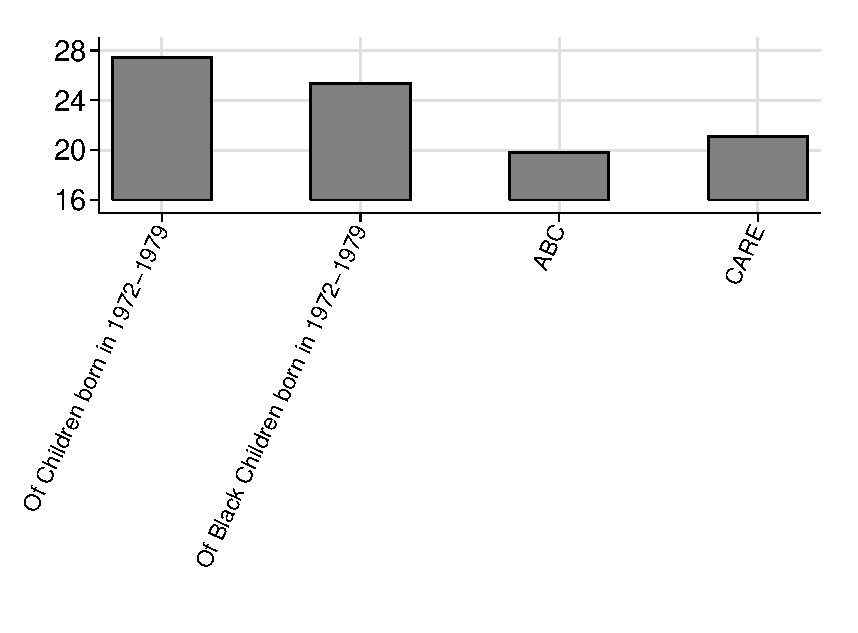
\includegraphics[width=20em]{output/abccarepsid_m_age0pool.eps}
\end{figure}
\end{frame}

%% ---------------------------------------------------------------------------

\begin{frame}
\frametitle{ABC and CARE Samples in Context}
\begin{figure}
\caption{Average Education of Mothers at Child's Birth}
	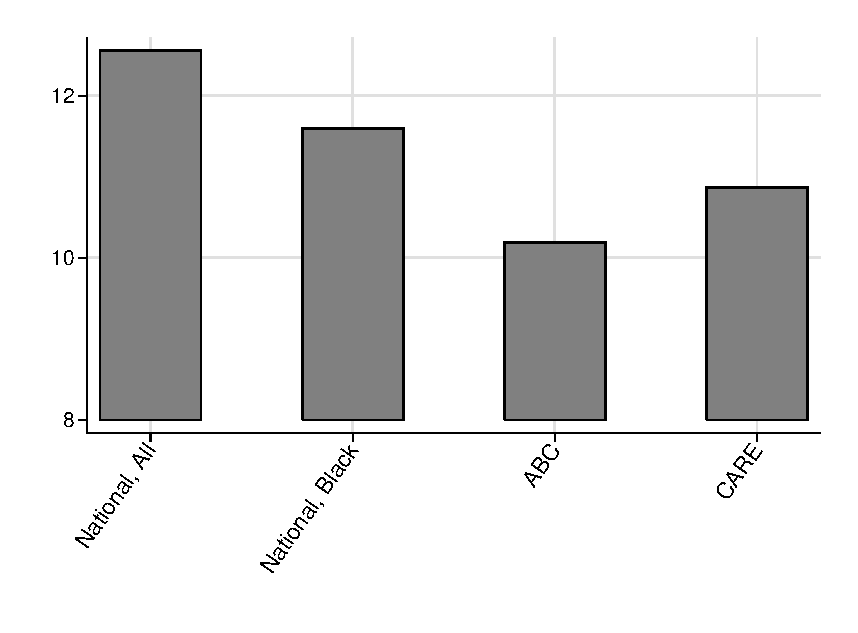
\includegraphics[width=20em]{output/abccarepsid_m_edu0pool.eps}
\end{figure}
\end{frame}

%% ---------------------------------------------------------------------------

\begin{frame}
\frametitle{ABC and CARE Samples in Context}
\begin{figure}
\caption{Proportion of Fathers at Home at Child's Birth}
	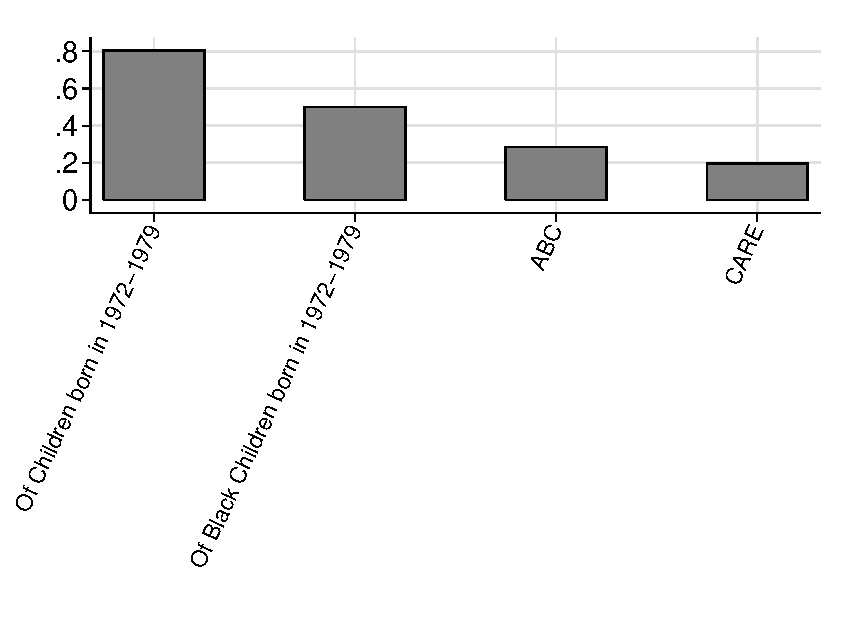
\includegraphics[width=20em]{output/abccarepsid_f_home0pool.eps}
\end{figure}
\end{frame}

%% ---------------------------------------------------------------------------

\begin{frame}
\frametitle{ABC Randomization}
	\begin{itemize}
		\item First Phase: 122 children randomized to one treatment group that received center-based childcare and one control group
		\begin{itemize}
			\item Effective sample size after randomization compromises: 116 (59 treatment, 57 control)
		\end{itemize}
		\item Second Phase: 96 of the original children were randomized into one treatment and one control group
	\end{itemize}
\end{frame}

%% ---------------------------------------------------------------------------

\begin{frame}
\frametitle{CARE Randomization}
	\begin{itemize}
		\item First Phase: 67 children randomized into:
		\begin{itemize}
			\item One treatment group that received center-based childcare and family education (16 children)
			\item One treatment group that only received family education (27 children)
			\item One control group (23 children)
		\end{itemize}
		\item Second Phase: Children in the two treatment groups automatically received the second-phase treatment and the control group remained the same
		\item No randomization compromises except death and families moving away from the study area
	\end{itemize}
\end{frame}

\begin{frame}\frametitle{ABC Fist-phase Randomization Compromises}
\begin{enumerate}
\item \textbf{Left the study before data collection:} We have no data at all for these subjects 
\item \textbf{Death before age 5 / Moved out:} We include them in estimations until data are no longer available. Thereafter, they are cases of attrition 
\item \textbf{Partial treatment:} We assume that they had full treatment
\item \textbf{Noncompliance to treatment:} We keep the original treatment status for them for ITT estimations
\item \textbf{Crossover from control to treatment:} Three children switched status from control to treatment. We keep the original treatment statuses for ITT estimations
\item \textbf{Developmental delays:} We drop them because they were not eligible for the program

\end{enumerate}
\end{frame}

%% ---------------------------------------------------------------------------

\begin{frame}
	\frametitle{ABC Second-phase Randomization Compromises}
	\begin{enumerate}
	\item \textbf{Not randomized in second phase:}
		\begin{itemize}
		\item \underline{Stopped being followed-up:} They are considered cases of attrition
		\item \underline{Followed-up in later data collection:} They are not included when calculating the treatment effects for the second phase, but are included when estimating treatment effects of the first phase on later outcomes
		\end{itemize}
	\item \textbf{Noncompliance in second phase:} Original treatment statuses are kept for ITT estimations
	\end{enumerate}
\end{frame}

%% ---------------------------------------------------------------------------

\begin{frame}
\frametitle{Programmatic Elements}
\begin{itemize}
\item The objectives of both ABC and CARE were to prevent ``mental retardation" and develop school readiness
\item The different curricula implemented across the programs and cohorts had the following goals:
	\begin{itemize}
		\item Support language and cognitive development
		\item Develop socio-emotional skills considered to enable school-readiness (e.g. task orientation)
	\end{itemize}
\end{itemize}
\end{frame}

%% ---------------------------------------------------------------------------

\begin{frame}
\frametitle{Additional Programmatic Elements}
\begin{itemize}
	\item The ABC treatment group received
	\begin{itemize}
		\item Daily health screenings and frequent medical check-ups 
	\end{itemize}
	\item The CARE treatment groups received
		\begin{itemize}
		\item Home visits to help parents foment problem-solving skills
		\end{itemize}
	\item Both ABC and CARE center-based treatment groups received
	\begin{itemize}
		\item Transportation to and from FPGC
		\item Daily nutritious food
	\end{itemize}
	\item Both ABC and CARE control groups received
	\begin{itemize}
		\item Iron-fortified formula until the child was 15 months old
		\item Unlimited diapers until the child was 3 years old
	\end{itemize}
\end{itemize}
\end{frame}

%% ---------------------------------------------------------------------------

\begin{frame}
\frametitle{Programmatic Elements, Second Phase}\label{elements}
\begin{itemize}	
	\item Same treatment in ABC and CARE
	\item State-certified ``home-school resource teachers" 
	\item Visited the elementary school and the children's homes twice a month to help
		\begin{itemize}
			\item Engage the parents with the children's academics
			\item Provide one-on-one tutoring to the children
			\item Parents with issues related to literacy, housing, and medical care
		\end{itemize}
\end{itemize}
\hyperlink{first_phase}{\beamergotobutton{Comparison}}
\end{frame}

%% ---------------------------------------------------------------------------

\begin{frame}
\frametitle{Baseline Characteristics in ABC and CARE}
\label{baseline_abccare}
	\begin{center}
	\begin{table}
	\caption{Baseline Characteristics in ABC and CARE}
	\scalebox{0.7}{\begin{table}[H]
\captionsetup{singlelinecheck=false,justification=centering}
\caption{Baseline Characteristics Comparison between ABC and CARE \label{tab:baseline}}

  \begin{threeparttable}
  \begin{tabular}{cccccccc} \toprule

     &  & \scriptsize{ABC} & \scriptsize{CARE} & \scriptsize{ABC} & \scriptsize{CARE} & \mc{2}{c}{\scriptsize{$p$-value}} \\  

    \scriptsize{Variable} & \scriptsize{Age} & \scriptsize{Obs} & \scriptsize{Obs} & \scriptsize{Mean} & \scriptsize{Mean} & \scriptsize{Single $H_0$} & \scriptsize{Multiple $H_0$} \\ 
    \hline  

    \mc{1}{l}{\scriptsize{Male}} & \mc{1}{c}{\scriptsize{0}} & \mc{1}{c}{\scriptsize{116}} & \mc{1}{c}{\scriptsize{67}} & \mc{1}{c}{\scriptsize{0.464}} & \mc{1}{c}{\scriptsize{0.596}} & \mc{1}{c}{\scriptsize{\textbf{(0.060)}}} & \mc{1}{c}{\scriptsize{(0.110)}} \\  

    \mc{1}{l}{\scriptsize{Birth Weight}} & \mc{1}{c}{\scriptsize{0}} & \mc{1}{c}{\scriptsize{114}} & \mc{1}{c}{\scriptsize{64}} & \mc{1}{c}{\scriptsize{7.008}} & \mc{1}{c}{\scriptsize{7.139}} & \mc{1}{c}{\scriptsize{(0.625)}} & \mc{1}{c}{\scriptsize{(0.765)}} \\  

    \mc{1}{l}{\scriptsize{No. Siblings in Household}} & \mc{1}{c}{\scriptsize{0}} & \mc{1}{c}{\scriptsize{116}} & \mc{1}{c}{\scriptsize{67}} & \mc{1}{c}{\scriptsize{0.632}} & \mc{1}{c}{\scriptsize{0.684}} & \mc{1}{c}{\scriptsize{(0.810)}} & \mc{1}{c}{\scriptsize{(0.890)}} \\  

    \mc{1}{l}{\scriptsize{Birth Year}} & \mc{1}{c}{\scriptsize{0}} & \mc{1}{c}{\scriptsize{116}} & \mc{1}{c}{\scriptsize{67}} & \mc{1}{c}{\scriptsize{1974}} & \mc{1}{c}{\scriptsize{1979}} & \mc{1}{c}{\scriptsize{\textbf{(0.000)}}} & \mc{1}{c}{\scriptsize{\textbf{(0.000)}}} \\ 
    \midrule

    \mc{1}{l}{\scriptsize{Mother's Education}} & \mc{1}{c}{\scriptsize{0}} & \mc{1}{c}{\scriptsize{116}} & \mc{1}{c}{\scriptsize{67}} & \mc{1}{c}{\scriptsize{10.188}} & \mc{1}{c}{\scriptsize{10.868}} & \mc{1}{c}{\scriptsize{\textbf{(0.010)}}} & \mc{1}{c}{\scriptsize{\textbf{(0.025)}}} \\  

    \mc{1}{l}{\scriptsize{Mother's Age}} & \mc{1}{c}{\scriptsize{0}} & \mc{1}{c}{\scriptsize{116}} & \mc{1}{c}{\scriptsize{67}} & \mc{1}{c}{\scriptsize{19.828}} & \mc{1}{c}{\scriptsize{21.141}} & \mc{1}{c}{\scriptsize{\textbf{(0.060)}}} & \mc{1}{c}{\scriptsize{\textbf{(0.100)}}} \\  

    \mc{1}{l}{\scriptsize{Mother's IQ}} & \mc{1}{c}{\scriptsize{0}} & \mc{1}{c}{\scriptsize{116}} & \mc{1}{c}{\scriptsize{67}} & \mc{1}{c}{\scriptsize{84.407}} & \mc{1}{c}{\scriptsize{87.164}} & \mc{1}{c}{\scriptsize{\textbf{(0.070)}}} & \mc{1}{c}{\scriptsize{(0.130)}} \\  

    \mc{1}{l}{\scriptsize{Father at Home}} & \mc{1}{c}{\scriptsize{0}} & \mc{1}{c}{\scriptsize{116}} & \mc{1}{c}{\scriptsize{67}} & \mc{1}{c}{\scriptsize{0.283}} & \mc{1}{c}{\scriptsize{0.209}} & \mc{1}{c}{\scriptsize{(0.270)}} & \mc{1}{c}{\scriptsize{(0.380)}} \\  

  \bottomrule
  \end{tabular}
    \begin{tablenotes}
    \scriptsize
    \item 
    Note: This table compares baseline, observed characteristics between ABC and CARE. 
    For each characteristic, we present the $p$-value from a single hypothesis test.
    We also present the $p$-values from multiple testing, where we collectively test the
    baseline characteristics within the blocks separated by the horizontal line.
    Both $p$-values are two-sided and non-parametric. We construct them 
    based on 1,000 re-draws of the full sample. The estimates we display are the means of 
    the empirical bootstrap distribution. 
    
    \end{tablenotes}
  \end{threeparttable}

\end{table}}
	\end{table}
	\end{center}
\hyperlink{sample}{\beamerreturnbutton{Back}}
\end{frame}

%% ---------------------------------------------------------------------------

\begin{frame}
\frametitle{Programmatic Elements, First Phase Treatment}
\label{first_phase}
	\begin{table}
		\caption{Elements of First Phase Treatment, ABC and CARE}
	\scalebox{0.55}{\begin{tabular}{L{4cm} L{7cm} L{7cm}} 
\toprule
& \multicolumn{1}{c}{ABC}& \multicolumn{1}{c}{CARE} \\
\midrule
\textbf{Treatment} & Center-based childcare & Center-based childcare and family education \\
\hspace{.5cm} \textbf{Center-based} \\
\hspace{.5cm} \textbf{Childcare} \\
\hspace{.5cm} Intensity &6.5--9.75 hours a day for 50 weeks per year& 6.5--9.75 hours a day for 50 weeks per year \\
\hspace{.5cm} Components & Instruction, medical care, nutrition, social services & Instruction, medical care, nutrition, social services \\
\hspace{.5cm} Staff-to-child Ratio &1:3 during ages 0--1 &1:3 during ages 0--1 \\
&1:4--5 during age 1--4 &1:4--5 during age 1--4 \\
&1:5--6 during ages 4--5 & 1:5--6 during ages 4--5 \\
\hspace{.5cm} Staff Qualifications &Mixed diplomas; experienced& Mixed diplomas; experienced \\ \\
\hspace{.5cm} \textbf{Family Education}  & \\
\hspace{.5cm} Intensity & & One hour-long home visits. 2--3 per month during ages 0--3. 1--2 per month during ages 4--5\\
\hspace{.5cm} Curriculum & & Social and mental stimulation; parent-child interaction\\
\hspace{.5cm} Staff-to-child Ratio & & 1:1\\
\hspace{.5cm} Staff Qualifications & & Home visitor training\\
\bottomrule
\end{tabular}}
	\end{table}
\end{frame}

%% ---------------------------------------------------------------------------

\begin{frame}
\frametitle{Programmatic Elements, Second Phase Treatment}
	\begin{table}
		\caption{Elements of Second Phase Treatment, ABC and CARE}
	\scalebox{0.6}{ \begin{tabular}{L{4cm} L{7cm} L{7cm}} 
\toprule
& \multicolumn{1}{c}{ABC}& \multicolumn{1}{c}{CARE}  \\ \midrule
\hspace{.5cm} Intensity &Every other week& Every other week \\
\hspace{.5cm} Components &Parent-teacher meetings& Parent-teacher meetings \\
\hspace{.5cm} Curriculum & Reading and math &  Reading and math \\
\hspace{.5cm} Staff-to-child Ratio &1:1& 1:1 \\
\hspace{.5cm} Staff Qualifications &Graduate degree and training in special education & Graduate degree and training in special education \\
\bottomrule
\end{tabular}}
	\end{table}
\hyperlink{programs}{\beamerreturnbutton{Back}}
\end{frame}

%% ---------------------------------------------------------------------------

\begin{frame}
\frametitle{Selection into Subsidized Alternative Preschools}\label{abc_subsidized}
\begin{figure}
\caption{Average Months in Treatment Substitution by Subsidized Status, ABC}
	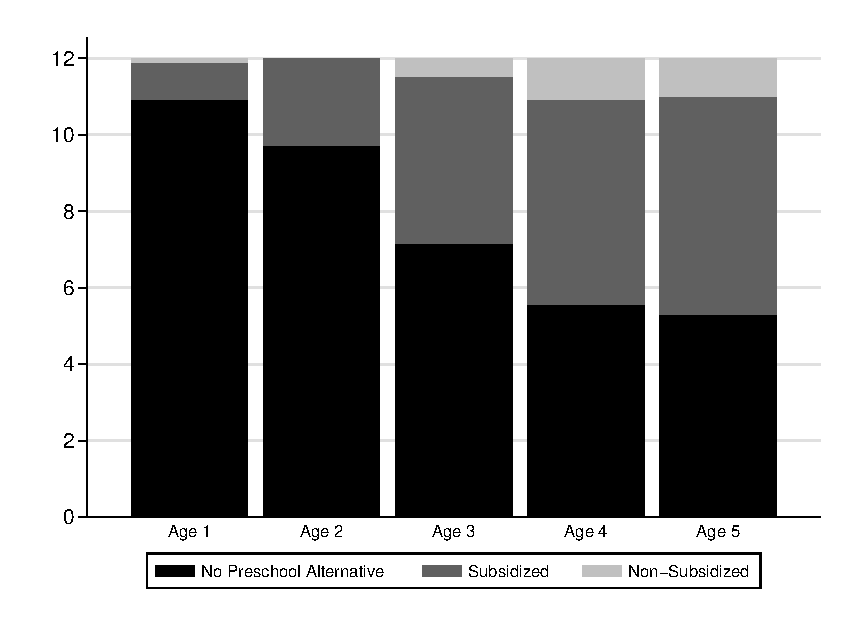
\includegraphics[width=18em]{output/blackwhite_CCnumber}
\end{figure}
\hyperlink{t_abc_substitution}{\beamerreturnbutton{Back}}
\end{frame}

%% ---------------------------------------------------------------------------

\begin{frame}
\frametitle{Selection into Subsidized Alternative Preschools}\label{care_subsidized}
\begin{figure}
\caption{Average Months in Treatment Substitution by Subsidized Status, CARE}
	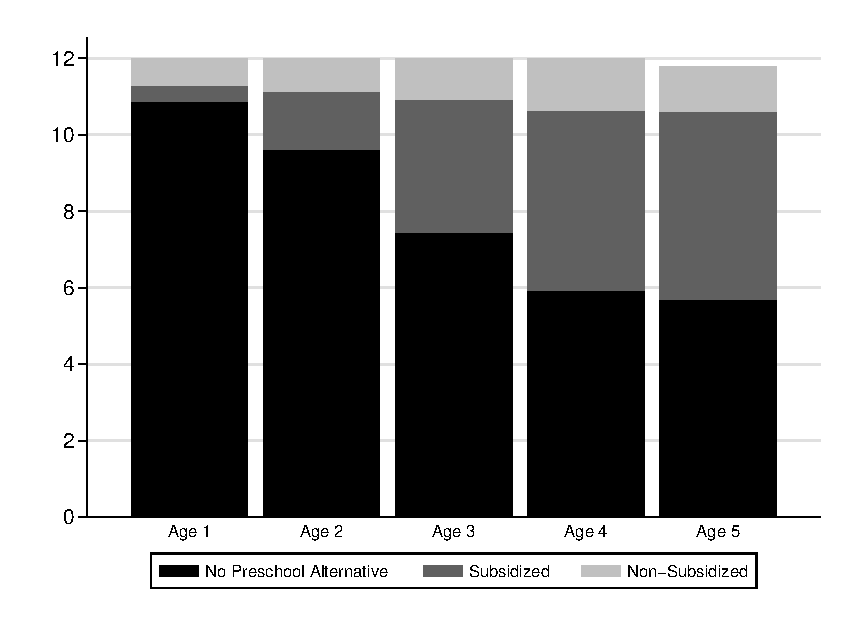
\includegraphics[width=18em]{output/blackwhite_CCnumber_care}
\end{figure}
\hyperlink{t_care_substitution}{\beamerreturnbutton{Back}}
\end{frame}

%% ---------------------------------------------------------------------------

\begin{frame}
\frametitle{Categorizing Outcomes as Socially Positive} \label{cat_outcomes}
\begin{itemize}
	\item Examples of socially positive outcomes
	\begin{itemize}
		\item Cognitive and achievement tests  
		\item Home environment measures
		\item Income
		\item Employment 
		\item Education 
	\end{itemize}
	\item Examples of socially negative outcomes (reversed)
	\begin{itemize}
		\item Public-transfer income
		\item Risky behavior
		\item Mental health issues
		\item Behavioral measures
		\item Health outcomes (e.g. blood pressure)
	\end{itemize}
\end{itemize}
\hyperlink{m_hypotheses}{\beamerreturnbutton{Back}}
\end{frame}

%% ---------------------------------------------------------------------------

\begin{frame}
\frametitle{Categorizing Outcomes as Socially Positive}
\begin{itemize}
	\item Examples of outcomes that are too ambiguous to categorize
	\begin{itemize}
		\item Number of children
		\item Age at birth of first child (apart from teenage pregnancy)
		\item Marriage status
		\item Car ownership
		\item Parenting style (authoritarian vs. progressive)
	\end{itemize}
\end{itemize}
\hyperlink{m_hypotheses}{\beamerreturnbutton{Back}}
\end{frame}

%% ---------------------------------------------------------------------------

\begin{frame} \label{stepdownfemales}

\frametitle{Treatment Effects on Females}
\begin{table}
	\caption{ABC and CARE Females, Selected Outcomes}
	\scalebox{0.8}{  \begin{tabular}{cccccccc}
  \toprule

    \scriptsize{Variable} & \scriptsize{Age} & \scriptsize{(1)} & \scriptsize{(2)} & \scriptsize{(3)} & \scriptsize{(4)} & \scriptsize{(5)} & \scriptsize{(6)} \\ 
    \midrule  

    \mc{1}{l}{\scriptsize{Std. IQ Test}} & \mc{1}{c}{\scriptsize{12}} & \mc{1}{c}{\scriptsize{8.688}} & \mc{1}{c}{\scriptsize{7.857}} & \mc{1}{c}{\scriptsize{6.850}} & \mc{1}{c}{\scriptsize{6.441}} & \mc{1}{c}{\scriptsize{9.120}} & \mc{1}{c}{\scriptsize{8.429}} \\  

     &  & \mc{1}{c}{\scriptsize{\textbf{(0.026)}}} & \mc{1}{c}{\scriptsize{\textbf{(0.053)}}} & \mc{1}{c}{\scriptsize{\textbf{(0.066)}}} & \mc{1}{c}{\scriptsize{\textbf{(0.092)}}} & \mc{1}{c}{\scriptsize{\textbf{(0.026)}}} & \mc{1}{c}{\scriptsize{\textbf{(0.053)}}} \\  

    \mc{1}{l}{\scriptsize{Years of Edu.}} & \mc{1}{c}{\scriptsize{30}} & \mc{1}{c}{\scriptsize{2.143}} & \mc{1}{c}{\scriptsize{1.695}} & \mc{1}{c}{\scriptsize{4.025}} & \mc{1}{c}{\scriptsize{3.918}} & \mc{1}{c}{\scriptsize{1.567}} & \mc{1}{c}{\scriptsize{1.409}} \\  

     &  & \mc{1}{c}{\scriptsize{\textbf{(0.000)}}} & \mc{1}{c}{\scriptsize{\textbf{(0.013)}}} & \mc{1}{c}{\scriptsize{\textbf{(0.000)}}} & \mc{1}{c}{\scriptsize{\textbf{(0.000)}}} & \mc{1}{c}{\scriptsize{\textbf{(0.026)}}} & \mc{1}{c}{\scriptsize{\textbf{(0.053)}}} \\  

    \mc{1}{l}{\scriptsize{Public-Transfer Income}} & \mc{1}{c}{\scriptsize{30}} & \mc{1}{c}{\scriptsize{-2,672}} & \mc{1}{c}{\scriptsize{-1,560}} & \mc{1}{c}{\scriptsize{-3,053}} & \mc{1}{c}{\scriptsize{-3,213}} & \mc{1}{c}{\scriptsize{-2,269}} & \mc{1}{c}{\scriptsize{-2,620}} \\  

     &  & \mc{1}{c}{\scriptsize{(0.158)}} & \mc{1}{c}{\scriptsize{(0.553)}} & \mc{1}{c}{\scriptsize{(0.145)}} & \mc{1}{c}{\scriptsize{\textbf{(0.092)}}} & \mc{1}{c}{\scriptsize{(0.342)}} & \mc{1}{c}{\scriptsize{(0.447)}} \\  

    \mc{1}{l}{\scriptsize{Employed}} & \mc{1}{c}{\scriptsize{30}} & \mc{1}{c}{\scriptsize{0.131}} & \mc{1}{c}{\scriptsize{0.080}} & \mc{1}{c}{\scriptsize{0.333}} & \mc{1}{c}{\scriptsize{0.340}} & \mc{1}{c}{\scriptsize{0.056}} & \mc{1}{c}{\scriptsize{0.070}} \\  

     &  & \mc{1}{c}{\scriptsize{(0.316)}} & \mc{1}{c}{\scriptsize{(0.632)}} & \mc{1}{c}{\scriptsize{(0.118)}} & \mc{1}{c}{\scriptsize{\textbf{(0.092)}}} & \mc{1}{c}{\scriptsize{(0.750)}} & \mc{1}{c}{\scriptsize{(0.724)}} \\  

    \mc{1}{l}{\scriptsize{Total Years Incarcerated}} & \mc{1}{c}{\scriptsize{30}} & \mc{1}{c}{\scriptsize{-0.024}} & \mc{1}{c}{\scriptsize{-0.025}} &  &  & \mc{1}{c}{\scriptsize{-0.037}} & \mc{1}{c}{\scriptsize{-0.038}} \\  

     &  & \mc{1}{c}{\scriptsize{(0.263)}} & \mc{1}{c}{\scriptsize{(0.276)}} &  &  & \mc{1}{c}{\scriptsize{(0.224)}} & \mc{1}{c}{\scriptsize{(0.289)}} \\  

    \mc{1}{l}{\scriptsize{Diabetes}} & \mc{1}{c}{\scriptsize{Mid-30s}} & \mc{1}{c}{\scriptsize{-0.071}} & \mc{1}{c}{\scriptsize{-0.032}} &  &  & \mc{1}{c}{\scriptsize{-0.091}} & \mc{1}{c}{\scriptsize{-0.095}} \\  

     &  & \mc{1}{c}{\scriptsize{(0.145)}} & \mc{1}{c}{\scriptsize{(0.342)}} &  &  & \mc{1}{c}{\scriptsize{(0.184)}} & \mc{1}{c}{\scriptsize{(0.118)}} \\  

  \bottomrule
  \end{tabular}}
\end{table}
\begin{tiny}
\leftright{\textbf{(1)} $\mathbb{E}_\Omega \big[ Y^1(\omega) - Y^0(\omega) | D = 1\big]$}{\textbf{(4)} $\mathbb{E}_\Omega \big[ Y^1(v, \omega) - Y^0(v, \omega) | V=0, D = 1 \big] $} \par
\leftright{\textbf{(2)} $\mathbb{E}_\Omega \big[ Y^1(\omega) - Y^0(\omega) |  X, D = 1 \big]$}{\textbf{(5)} $\mathbb{E}_\Omega \big[ Y^1(\omega) \big] - \mathbb{E}_\Omega \big[ Y^0(v, \omega) | V > 0, D =1 \big]$} \par
\leftright{\textbf{(3)} $\mathbb{E}_\Omega \big[ Y^1(\omega) \big] - \mathbb{E}_\Omega \big[ Y^0(v, \omega) | V =0, D =1 \big]$}{\textbf{(6)} $\mathbb{E}_\Omega \big[ Y^1(v, \omega) - Y^0(v, \omega) | V > 0 , D = 1\big]$}

\end{tiny}
\hyperlink{resultsfemales}{\beamergotobutton{Back}}
\end{frame}

%% ---------------------------------------------------------------------------

\begin{frame} \label{stepdownmales}
\frametitle{Treatment Effects on Males}
\begin{table}
	\caption{ABC and CARE Males, Selected Outcomes}
	\scalebox{0.7}{  \begin{tabular}{cccccccc}
  \toprule

    \scriptsize{Variable} & \scriptsize{Age} & \scriptsize{(1)} & \scriptsize{(2)} & \scriptsize{(3)} & \scriptsize{(4)} & \scriptsize{(5)} & \scriptsize{(6)} \\ 
    \midrule  

    \mc{1}{l}{\scriptsize{Years of Edu.}} & \mc{1}{c}{\scriptsize{30}} & \mc{1}{c}{\scriptsize{0.525}} & \mc{1}{c}{\scriptsize{0.708}} & \mc{1}{c}{\scriptsize{0.857}} & \mc{1}{c}{\scriptsize{0.791}} & \mc{1}{c}{\scriptsize{0.385}} & \mc{1}{c}{\scriptsize{0.347}} \\  

     &  & \mc{1}{c}{\scriptsize{(0.316)}} & \mc{1}{c}{\scriptsize{(0.263)}} & \mc{1}{c}{\scriptsize{(0.303)}} & \mc{1}{c}{\scriptsize{(0.303)}} & \mc{1}{c}{\scriptsize{(0.500)}} & \mc{1}{c}{\scriptsize{(0.579)}} \\  

    \mc{1}{l}{\scriptsize{Labor Income}} & \mc{1}{c}{\scriptsize{30}} & \mc{1}{c}{\scriptsize{19,810}} & \mc{1}{c}{\scriptsize{24,902}} & \mc{1}{c}{\scriptsize{17,909}} & \mc{1}{c}{\scriptsize{24,012}} & \mc{1}{c}{\scriptsize{20,065}} & \mc{1}{c}{\scriptsize{21,170}} \\  

     &  & \mc{1}{c}{\scriptsize{(0.355)}} & \mc{1}{c}{\scriptsize{(0.618)}} & \mc{1}{c}{\scriptsize{(0.355)}} & \mc{1}{c}{\scriptsize{(0.303)}} & \mc{1}{c}{\scriptsize{(0.316)}} & \mc{1}{c}{\scriptsize{(0.395)}} \\  

    \mc{1}{l}{\scriptsize{Employed}} & \mc{1}{c}{\scriptsize{30}} & \mc{1}{c}{\scriptsize{0.119}} & \mc{1}{c}{\scriptsize{0.179}} & \mc{1}{c}{\scriptsize{-0.029}} & \mc{1}{c}{\scriptsize{0.041}} & \mc{1}{c}{\scriptsize{0.176}} & \mc{1}{c}{\scriptsize{0.262}} \\  

     &  & \mc{1}{c}{\scriptsize{(0.395)}} & \mc{1}{c}{\scriptsize{(0.276)}} & \mc{1}{c}{\scriptsize{(0.921)}} & \mc{1}{c}{\scriptsize{(0.868)}} & \mc{1}{c}{\scriptsize{(0.276)}} & \mc{1}{c}{\scriptsize{\textbf{(0.079)}}} \\  

    \mc{1}{l}{\scriptsize{Total Misdemeanor Arrests}} & \mc{1}{c}{\scriptsize{Mid-30s}} & \mc{1}{c}{\scriptsize{-0.501}} & \mc{1}{c}{\scriptsize{-0.239}} & \mc{1}{c}{\scriptsize{-0.251}} & \mc{1}{c}{\scriptsize{-0.040}} & \mc{1}{c}{\scriptsize{-0.665}} & \mc{1}{c}{\scriptsize{-0.512}} \\  

     &  & \mc{1}{c}{\scriptsize{(0.368)}} & \mc{1}{c}{\scriptsize{(0.592)}} & \mc{1}{c}{\scriptsize{(0.724)}} & \mc{1}{c}{\scriptsize{(0.750)}} & \mc{1}{c}{\scriptsize{(0.289)}} & \mc{1}{c}{\scriptsize{(0.303)}} \\  

    \mc{1}{l}{\scriptsize{Diastolic Blood Pressure (mm Hg)}} & \mc{1}{c}{\scriptsize{Mid-30s}} & \mc{1}{c}{\scriptsize{-10.854}} & \mc{1}{c}{\scriptsize{-19.895}} & \mc{1}{c}{\scriptsize{-8.640}} & \mc{1}{c}{\scriptsize{-8.150}} & \mc{1}{c}{\scriptsize{-14.240}} & \mc{1}{c}{\scriptsize{-21.851}} \\  

     &  & \mc{1}{c}{\scriptsize{\textbf{(0.039)}}} & \mc{1}{c}{\scriptsize{\textbf{(0.013)}}} & \mc{1}{c}{\scriptsize{(0.116)}} & \mc{1}{c}{\scriptsize{(0.130)}} & \mc{1}{c}{\scriptsize{\textbf{(0.066)}}} & \mc{1}{c}{\scriptsize{\textbf{(0.026)}}} \\  

    \mc{1}{l}{\scriptsize{Vitamin D Deficiency}} & \mc{1}{c}{\scriptsize{Mid-30s}} & \mc{1}{c}{\scriptsize{-0.245}} & \mc{1}{c}{\scriptsize{-0.185}} & \mc{1}{c}{\scriptsize{-0.480}} & \mc{1}{c}{\scriptsize{-0.485}} & \mc{1}{c}{\scriptsize{-0.172}} & \mc{1}{c}{\scriptsize{-0.189}} \\  

     &  & \mc{1}{c}{\scriptsize{\textbf{(0.066)}}} & \mc{1}{c}{\scriptsize{(0.132)}} & \mc{1}{c}{\scriptsize{\textbf{(0.000)}}} & \mc{1}{c}{\scriptsize{\textbf{(0.000)}}} & \mc{1}{c}{\scriptsize{(0.158)}} & \mc{1}{c}{\scriptsize{(0.158)}} \\  

    \mc{1}{l}{\scriptsize{Self-reported drug user}} & \mc{1}{c}{\scriptsize{Mid-30s}} & \mc{1}{c}{\scriptsize{-0.333}} & \mc{1}{c}{\scriptsize{-0.432}} & \mc{1}{c}{\scriptsize{-0.500}} & \mc{1}{c}{\scriptsize{-0.555}} & \mc{1}{c}{\scriptsize{-0.233}} & \mc{1}{c}{\scriptsize{-0.330}} \\  

     &  & \mc{1}{c}{\scriptsize{\textbf{(0.066)}}} & \mc{1}{c}{\scriptsize{\textbf{(0.000)}}} & \mc{1}{c}{\scriptsize{(0.105)}} & \mc{1}{c}{\scriptsize{\textbf{(0.092)}}} & \mc{1}{c}{\scriptsize{(0.355)}} & \mc{1}{c}{\scriptsize{(0.158)}} \\  

  \bottomrule
  \end{tabular}}
\end{table}
\begin{tiny}
\leftright{\textbf{(1)} $\mathbb{E}_\Omega \big[ Y^1(\omega) - Y^0(\omega) | D = 1\big]$}{\textbf{(4)} $\mathbb{E}_\Omega \big[ Y^1(v, \omega) - Y^0(v, \omega) | V=0, D = 1 \big] $} \par
\leftright{\textbf{(2)} $\mathbb{E}_\Omega \big[ Y^1(\omega) - Y^0(\omega) |  X, D = 1 \big]$}{\textbf{(5)} $\mathbb{E}_\Omega \big[ Y^1(\omega) \big] - \mathbb{E}_\Omega \big[ Y^0(v, \omega) | V > 0, D =1 \big]$} \par
\leftright{\textbf{(3)} $\mathbb{E}_\Omega \big[ Y^1(\omega) \big] - \mathbb{E}_\Omega \big[ Y^0(v, \omega) | V =0, D =1 \big]$}{\textbf{(6)} $\mathbb{E}_\Omega \big[ Y^1(v, \omega) - Y^0(v, \omega) | V > 0 , D = 1\big]$}

\end{tiny}
\hyperlink{resultsmales}{\beamergotobutton{Back}}
\end{frame}

%% ---------------------------------------------------------------------------

\begin{frame} \label{components}

\frametitle{Components of the CBA}

We incorporate all the categories of outcomes we are able to monetize

\begin{itemize}

	\item Program costs for treatment and control groups

	\item Costs of alternative preschool arrangements for the control group

	\item Savings due to reduced grade retention, special education

	\item Costs due to post-secondary schooling

	\item Parental income

\end{itemize}

(cont.)

\end{frame}





%% ---------------------------------------------------------------------------



\begin{frame}

\label{components}

\frametitle{Components of the CBA}

\begin{itemize}

	\item Subject labor income

	\item Subject public transfer income

	\item Medical expenditure 

	\item QALY

	\item Crime

\end{itemize}

\end{frame}



%% ---------------------------------------------------------------------------

\begin{frame}

\frametitle{Components of the CBA}

		

\begin{itemize}

\item Costs of education are estimated based on literature standards \citep[e.g.][]{Snyder_Willow_2012_BOOK_NCES}

\item Cognitive, noncognitive, and scholastic gains we are unable to monetize are assumed to enter into the other components of the analysis

\item Educational attainment is observed up to age 30 and assumed to remain

 constant

\end{itemize}

\end{frame}



Note: All monetary values are presented in 2014 USD.

\clearpage



%% ---------------------------------------------------------------------------

\begin{frame}

\frametitle{Program Costs}

%We approximate the cost of the program using four categories:

Medical costs

	\begin{itemize}

		\item Regular check-ups by full-time pediatric fellows and nurses

		\item Excludes laboratory costs 

	\end{itemize}

Non-medical labor costs

	\begin{itemize}

		\item Salaries of classroom staff, administrative staff, and support staff (e.g. transportation providers)

	\end{itemize}

Other costs

	\begin{itemize}

		\item Costs of transportation provided by the center, nutrition, and curricular materials

	\end{itemize}

\end{frame}



%% ---------------------------------------------------------------------------

\begin{frame}

\frametitle{Program Costs}



\begin{table}

\begin{center}

\caption{Individual Program Costs by Group}

\scalebox{.5}{
\begin{tabular}{lc} \toprule
\multicolumn{1}{c}{Item} & Yearly Cost in 2014 USD \\ \midrule
1 Program Director & $60,935$ \\ 
1 Social Worker      &  $35,869$ \\ 
3 Lead Teachers and 2 Teachers Aides (Nursery)  & $204,457$ \\
4 Lead Teachers and 4 Teacher Aides  (Toddlers) & $305,181$ \\ 
2 Teaching Support Staff & $53,341$ \\ 
1 Secretary & $32,973$ \\ 
1 Clerk        & $32,537$ \\ 
Workers' Fringe Benefits & $124,935$ \\ 
Other & $4, 891$ \\ \\ \midrule 
Total  & $962,726$ \\ 
Total per Subject & $18,514$ \\ \bottomrule
\end{tabular}}

\end{center}

\end{table}

{\tiny\flushleft Note: This table summarizes the yearly costs for ABC and CARE. They are based on primary-source documentation describing ABC. We assume that the costs for ABC and CARE were the same based on conversations with programs' staff \citet{projectcare2014interviews,abc2014-2015interviews}.}

\hyperlink{costs}{\beamergotobutton{Back}}		

\end{frame}
\backupend

%% ---------------------------------------------------------------------------

%%
%%--------------------------- Content ends here ---------------------------------------------------
%%

% --------------------- Bibliography hidden with a save box ---------------------------------------
\mode<all>
\bibliographystyle{chicago}
\savebox\hiddenbib{\parbox{\textwidth}{\bibliography{heckman}}}

\end{document} 